\chapter{DESAIN DAN IMPLEMENTASI}
\label{chap:desainimplementasi}

\section{Analisis Kebutuhan}
\begin{figure}[H]
    \centering
    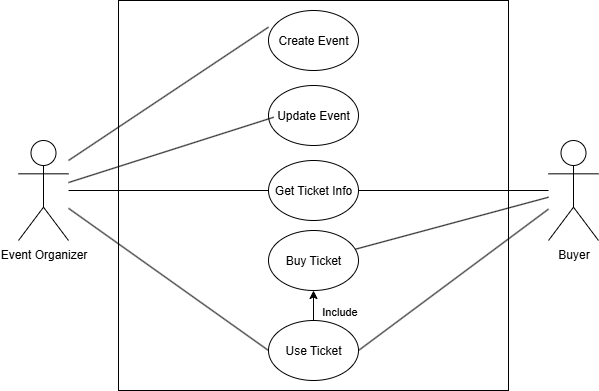
\includegraphics[width=.6\textwidth]{gambar/bab3/usecase.png}
    \caption{Diagram \emph{usecase}}
    \label{fig:usecase}
\end{figure}
Sistem Ticket Marketplace yang dikembangkan dalam penelitian ini memerlukan
fungsi utama yang mendukung operasional pasar tiket digital berbasis
blockchain. Kebutuhan fungsional ini diidentifikasi berdasarkan analisis
terhadap karakteristik fundamental dari sistem tiket tradisional yang
ditransformasikan ke dalam paradigma implementasi berbasis desentralisasi dan
NFT. Setiap fungsi dirancang untuk memenuhi ekspektasi pengguna dalam ekosistem
pasar digital sambil memanfaatkan keunggulan teknologi blockchain untuk
transparansi, kekekalan, dan tata kelola yang terdesentralisasi.

Implementasi fungsi manajemen event merupakan fondasi dari seluruh ekosistem
pasar, dimana penyelenggara event harus dapat membuat, mengatur, dan mengelola
event mereka dengan infrastruktur yang memadai. Fungsi createEvent dalam smart
contract dirancang untuk menerima parameter komprehensif yang mencakup aspek
operasional dan komersial dari acara, dengan mekanisme validasi yang memastikan
integritas data dan kepatuhan terhadap aturan bisnis yang telah ditetapkan.
Sistem otorisasi berbasis peran memungkinkan delegasi tanggung jawab manajemen
kepada tim yang berbeda, sementara jejak audit yang tidak dapat diubah
memberikan transparansi penuh terhadap seluruh perubahan yang dilakukan pada
konfigurasi acara.

Sistem pembelian tiket dirancang untuk memberikan pengalaman pengguna yang
lancar dan aman, dengan memanfaatkan keunggulan blockchain untuk menghilangkan
perantara dan pengurangan biaya transaksi. Fungsi purchaseTicket
mengimplementasikan mekanisme transaksi atom yang memastikan bahwa pembayaran
dan transfer kepemilikan tiket terjadi secara bersamaan tanpa kemungkinan
kegagalan sebagian. Sistem reservasi sementara menggunakan mekanisme
time-locked untuk memberikan window pembayaran yang memadai sambil mencegah
pemblokiran inventaris yang dapat merugikan ketersediaan untuk pengguna lain.
Proses pembuatan NFT mengintegrasikan metadata komprehensif yang mencakup
detail acara, informasi kursi, stempel waktu pembelian, dan bukti kriptografi
yang memungkinkan verifikasi independen tanpa bergantung pada otoritas
terpusat. Integrasi dengan solusi dompet populer memastikan kompatibilitas
dengan infrastruktur pengguna yang ada, sementara mekanisme fallback memberikan
metode akses alternatif untuk pengguna dengan kemampuan teknis berbeda.

Sistem validasi tiket merupakan komponen penting yang memastikan integritas dan
keamanan seluruh ekosistem pasar. Mekanisme validasi implementasi harus
menyeimbangkan antara persyaratan keamanan dan efisiensi operasional,
memungkinkan verifikasi cepat di titik masuk acara tanpa menimbulkan kemacetan
yang dapat mengganggu pengalaman peserta. Fungsi useTicket dalam \emph{smart
    contract} mengimplementasikan verifikasi kriptografi yang memvalidasi
kepemilikan, keaslian, dan status terkini dari tiket secara real-time melalui
query blockchain. Validasi jendela waktu memastikan bahwa tiket hanya dapat
digunakan dalam periode yang sesuai sekitar jadwal acara, mencegah penggunaan
penipuan di luar jangka waktu yang sah. Kemampuan integrasi dengan sistem
manajemen acara yang ada memungkinkan penggabungan yang mulus ke dalam alur
kerja operasional yang sudah ditetapkan, sementara antarmuka ramah seluler
memastikan aksesibilitas untuk staf venue dengan berbagai tingkat keahlian
teknis.

\section{Perancangan Sistem}
\subsection{Arsitektur Sistem}
\begin{figure}[H]
    \centering
    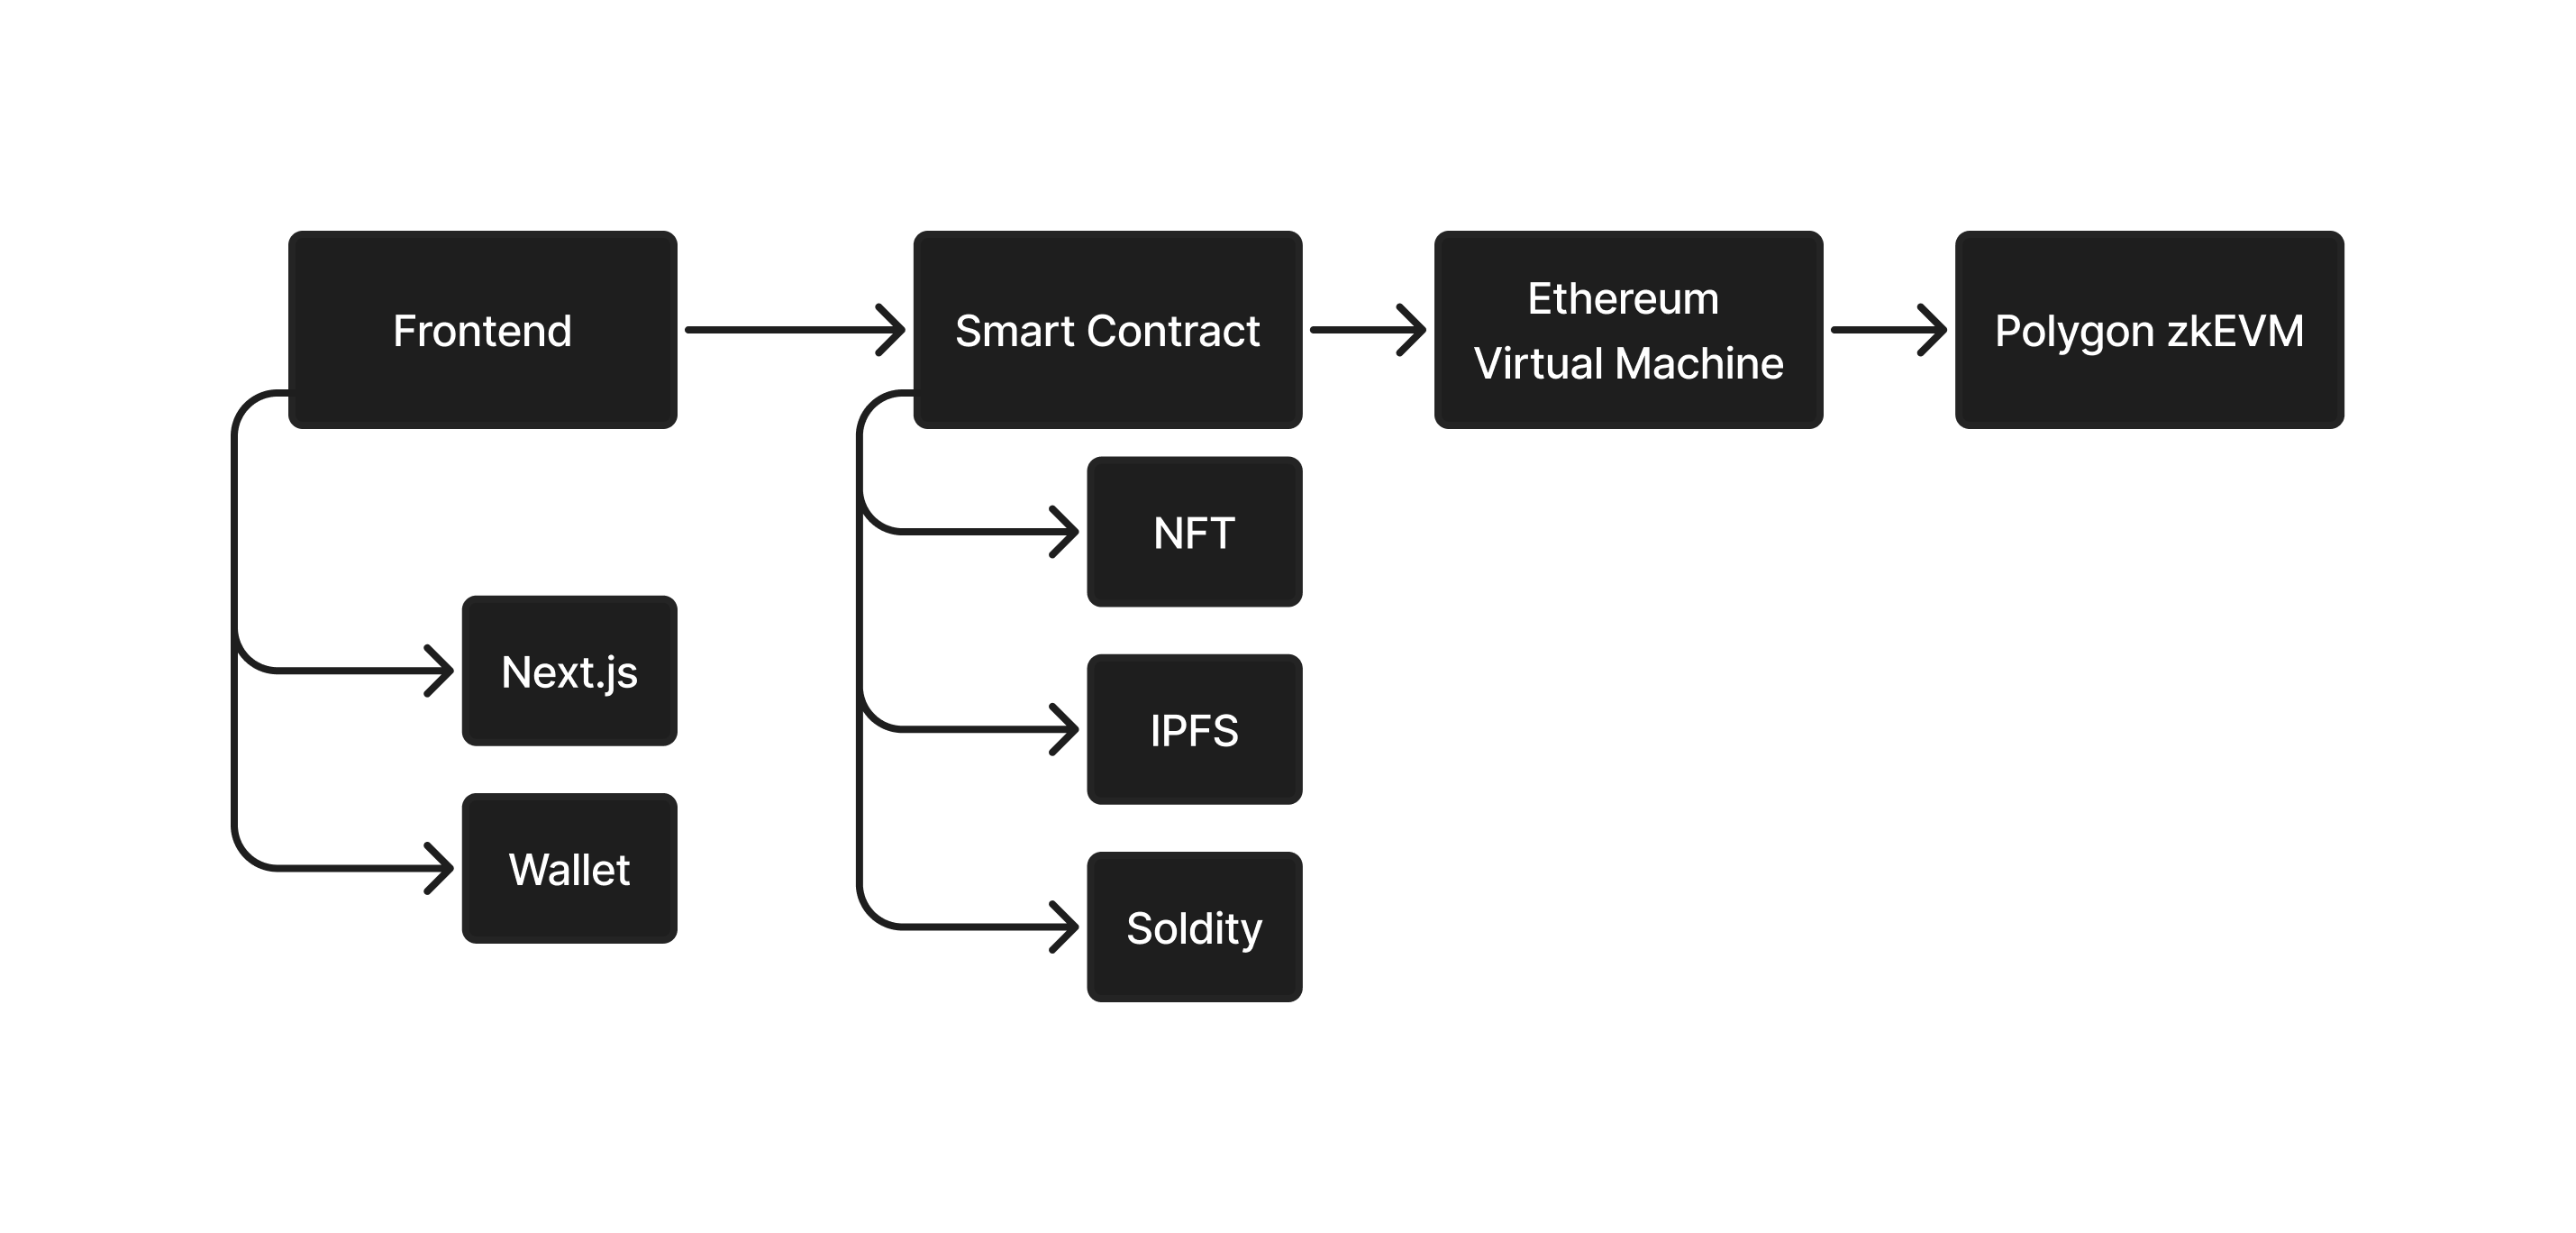
\includegraphics[width=.9\textwidth]{gambar/bab3/Untitled (2).png}
    \caption{Arsitektur Sistem}
    \label{fig:arsitektur}
\end{figure}
Arsitektur sistem yang dibangun dalam penelitian ini merupakan implementasi dari platform marketplace tiket konser berbasis teknologi blockchain dengan pendekatan terdesentralisasi. Sistem ini dirancang agar dapat mengelola proses pembuatan event, distribusi tiket, transaksi pembelian, serta validasi keaslian tiket melalui \emph{smart contract} berbasis Ethereum Virtual Machine (EVM). Guna meningkatkan efisiensi dan mengurangi biaya gas, sistem diimplementasikan di jaringan Polygon zkEVM, sebuah solusi Layer-2 Ethereum yang menggunakan teknologi Zero-Knowledge Rollup untuk menghadirkan performa tinggi dengan tetap mempertahankan kompatibilitas penuh terhadap EVM. Platform ini terdiri dari beberapa komponen utama yang saling terintegrasi, yaitu frontend berbasis web, wallet kripto, \emph{smart contract} berbasis NFT, penyimpanan metadata di IPFS, dan jaringan blockchain tempat \emph{smart contract} dijalankan.

Komponen frontend berfungsi sebagai antarmuka utama antara pengguna dan sistem.
Dalam penelitian ini, frontend dikembangkan menggunakan framework Next.js, yang
memungkinkan pengembangan aplikasi web dengan performa tinggi dan dukungan
render sisi server (server-side rendering) maupun sisi klien (client-side
rendering). Next.js dipilih karena fleksibilitasnya dalam membangun aplikasi
web modern berbasis React, yang dapat dengan mudah diintegrasikan dengan wallet
kripto seperti MetaMask. Melalui frontend ini, pengguna dapat melakukan
berbagai interaksi, seperti melihat daftar event, membeli tiket, menghubungkan
wallet, serta memverifikasi tiket yang dimiliki. Frontend juga menangani
permintaan pengguna dan meneruskannya ke \emph{smart contract} yang berjalan di
jaringan blockchain, serta menampilkan hasil transaksi yang telah dikonfirmasi.

Agar transaksi dapat dilakukan secara aman dan terdesentralisasi, sistem
terintegrasi dengan wallet seperti MetaMask, yang digunakan oleh pengguna untuk
menandatangani transaksi menggunakan kunci pribadi mereka. Wallet ini berfungsi
sebagai penghubung antara frontend dan jaringan blockchain, memastikan bahwa
semua transaksi, mulai dari pembelian hingga validasi tiket, dilakukan langsung
oleh pemilik akun tanpa perantara. Wallet juga memastikan bahwa pengguna
memiliki saldo yang cukup dan menyetujui kontrak sebelum melakukan interaksi.
Dengan pendekatan ini, sistem menjamin keaslian dan non-repudiation dari setiap
transaksi, karena seluruh aktivitas tercatat secara permanen di blockchain.

Sisi backend dari sistem digantikan oleh \emph{smart contract} yang ditulis
dalam bahasa pemrograman Solidity, yang merupakan bahasa standar untuk
pengembangan \emph{Smart Contract} di Ethereum. \emph{Smart contract} ini
mencakup logika utama dari sistem, seperti pembuatan event oleh penyelenggara
konser, pencetakan tiket dalam bentuk Non-Fungible Token (NFT) berbasis standar
ERC-721, serta fungsi untuk membeli dan memverifikasi tiket. NFT dipilih karena
karakteristiknya yang unik dan tidak dapat diduplikasi, menjadikannya ideal
sebagai representasi digital dari tiket konser. Untuk menyimpan data deskriptif
tiket, seperti nama event, lokasi, waktu, dan atribut visual lainnya, sistem
menggunakan IPFS (InterPlanetary File System) sebagai penyimpanan metadata
terdesentralisasi. IPFS memungkinkan distribusi file secara peer-to-peer yang
tahan sensor, efisien, dan cocok untuk digunakan bersama NFT.

\emph{Smart contract} yang telah dikembangkan dan diuji kemudian dideploy ke Ethereum
Virtual Machine (EVM), namun bukan di jaringan Layer-1 Ethereum, melainkan di
jaringan Polygon zkEVM. Polygon zkEVM dipilih karena merupakan solusi
skalabilitas yang menawarkan biaya transaksi rendah dan kecepatan tinggi,
sembari tetap mempertahankan keamanan dan kompatibilitas dengan EVM. Teknologi
zk-Rollup memungkinkan transaksi diproses secara off-chain, kemudian
digabungkan dan diverifikasi secara on-chain melalui bukti Zero-Knowledge.
Dengan demikian, sistem yang dibangun mampu menangani transaksi dalam jumlah
besar dengan efisiensi yang jauh lebih tinggi dibandingkan jaringan Layer-1
Ethereum, menjadikannya ideal untuk platform tiket konser yang memiliki potensi
lalu lintas tinggi.

Secara keseluruhan, integrasi antara frontend, wallet, \emph{smart contract},
IPFS, dan jaringan zkEVM membentuk sistem yang end-to-end terdesentralisasi,
transparan, dan aman. Setiap tiket yang dibeli oleh pengguna akan tercatat di
blockchain dalam bentuk NFT yang tidak dapat diubah, dimanipulasi, atau
dipalsukan. Metadata tiket disimpan secara aman di IPFS, dan validasi tiket
dilakukan secara langsung di \emph{smart contract} tanpa perlu kepercayaan
terhadap pihak ketiga. Dengan pendekatan ini, penelitian ini tidak hanya
membangun sistem yang fungsional, tetapi juga menunjukkan bagaimana teknologi
blockchain, khususnya pada jaringan Layer-2 Ethereum seperti Polygon zkEVM,
dapat dimanfaatkan untuk membangun platform digital yang lebih efisien,
terbuka, dan tahan terhadap manipulasi.

\subsection{Alur Sistem}
\begin{figure}[H]
    \centering
    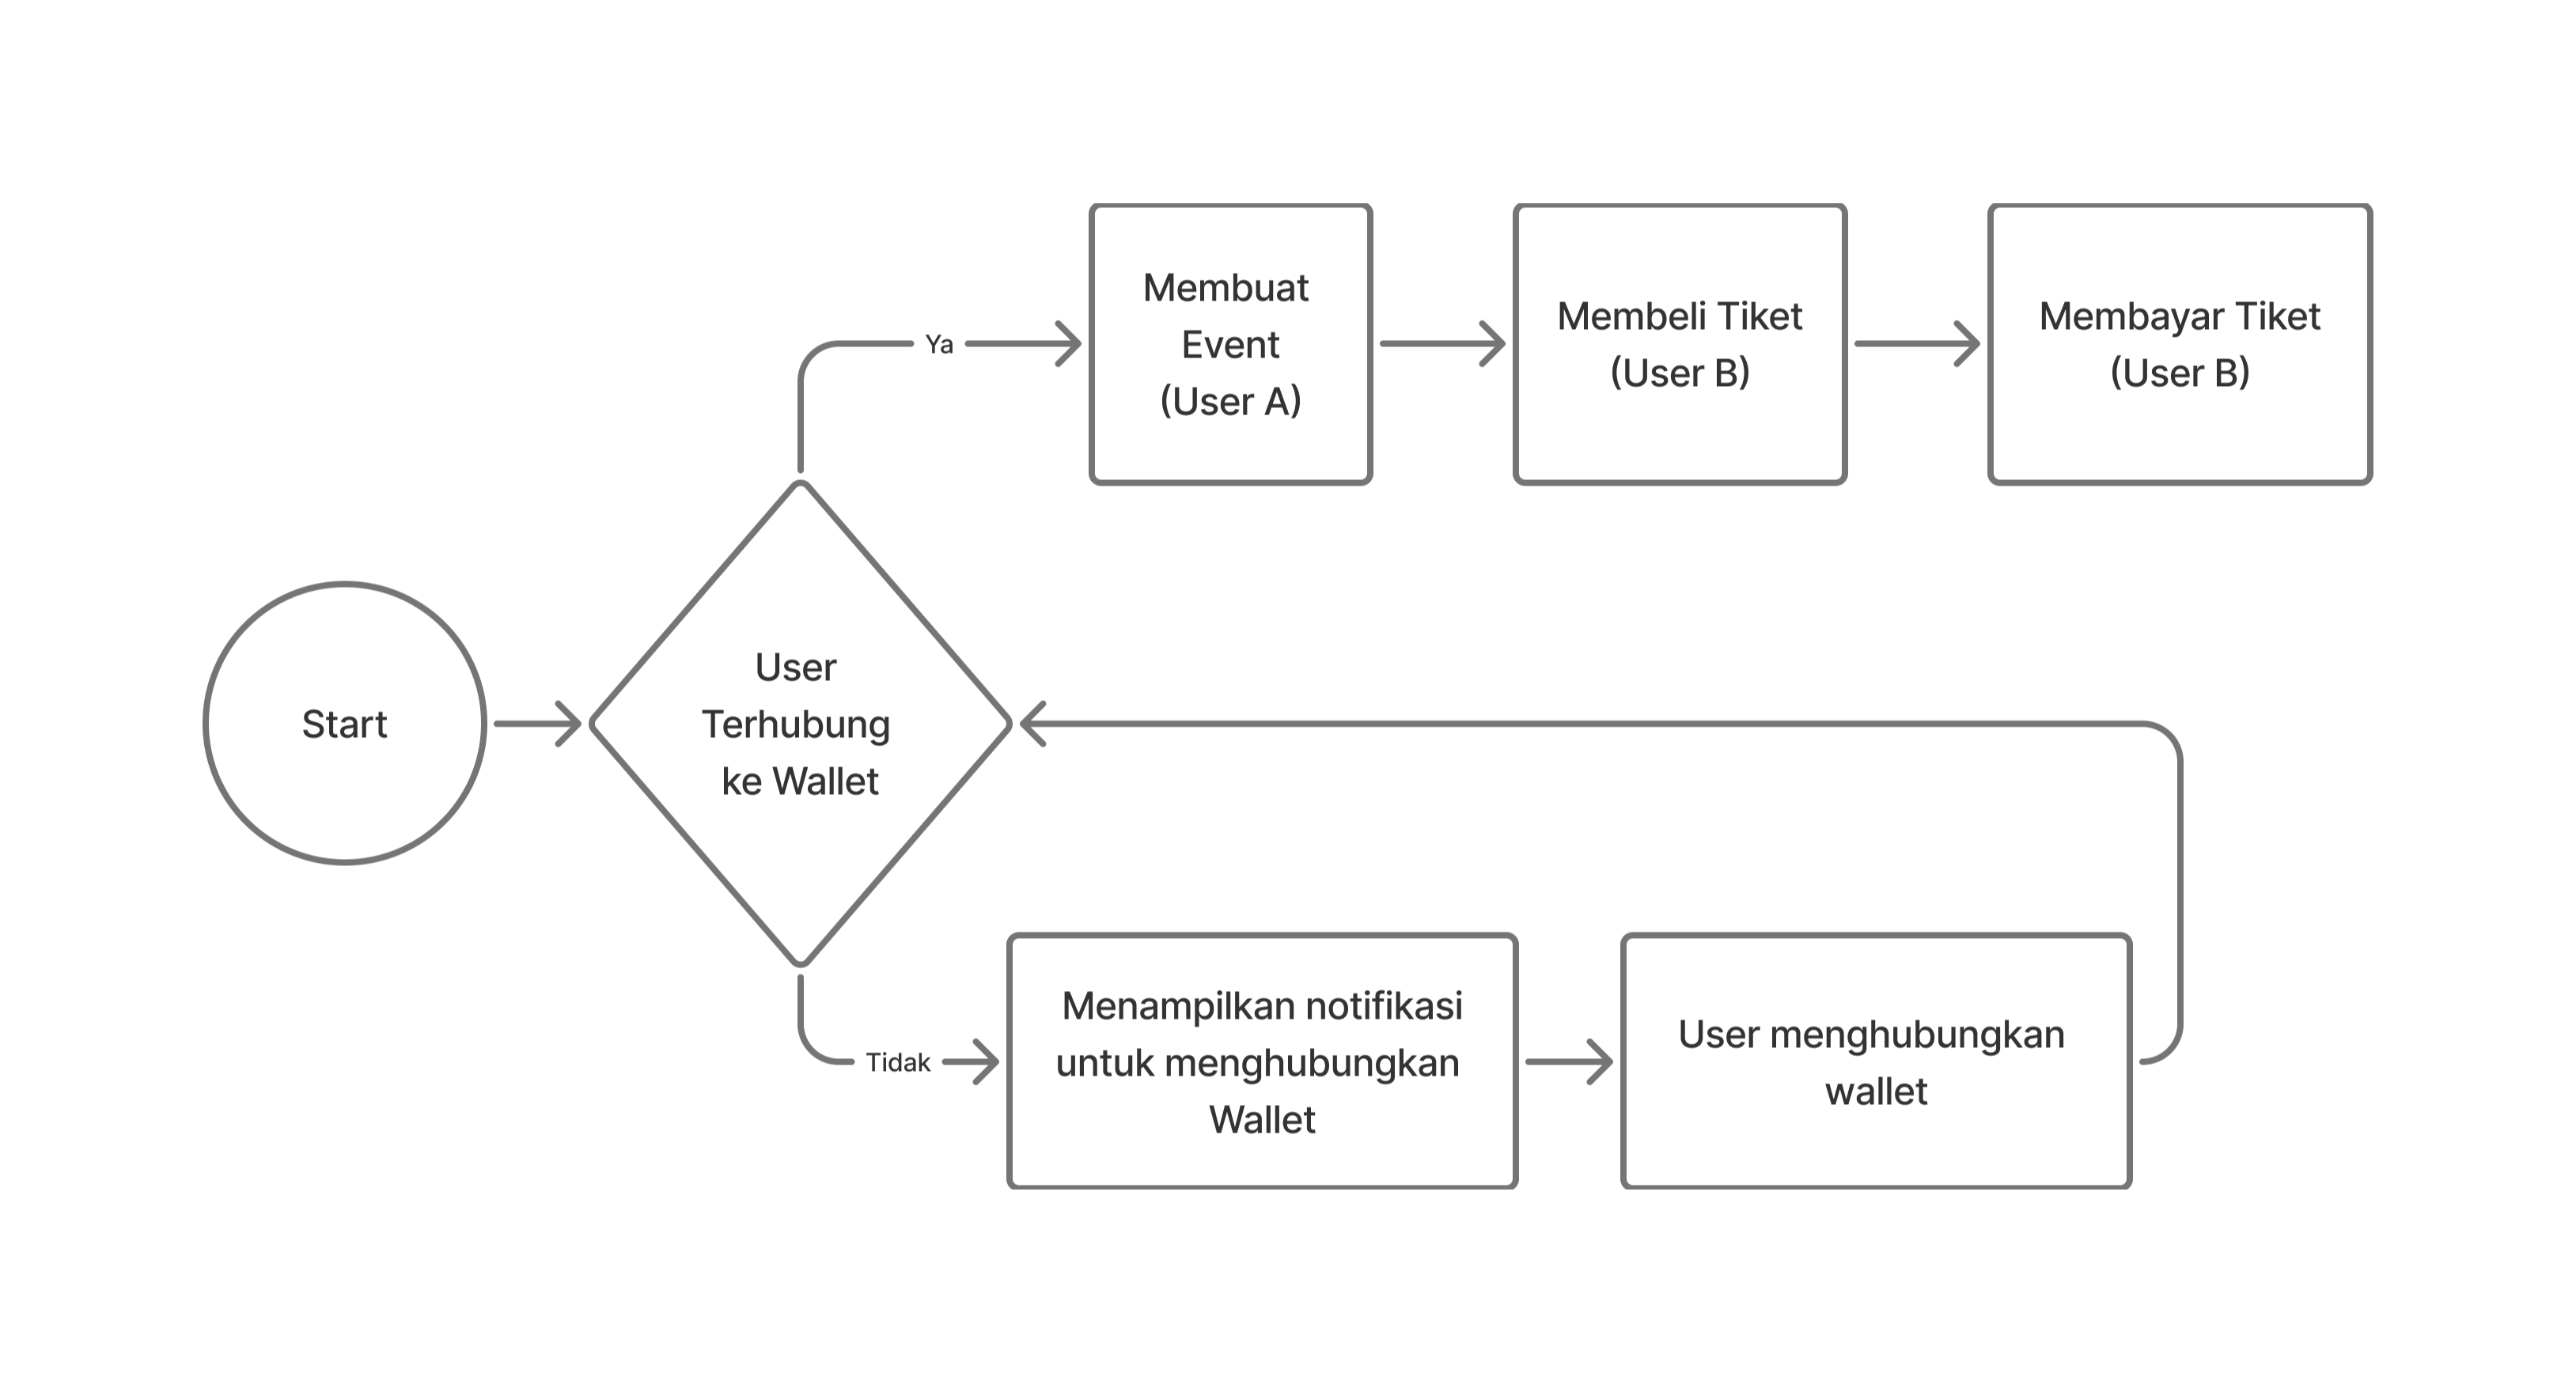
\includegraphics[width=.9\textwidth]{gambar/bab3/Untitled (4).png}
    \caption{Integrasi Wallet dan Proses Transaksional dalam DApp TicketMarketplace}
    \label{fig:flow-1}
\end{figure}
Gambar \ref{fig:flow-1} menampilkan diagram alur komprehensif yang mengilustrasikan proses integrasi \emph{wallet} dan aliran \emph{transaction} ujung ke ujung dalam aplikasi terdesentralisasi (\emph{DApp}) \emph{TicketMarketplace}, menunjukkan bagaimana pengguna berinteraksi dengan infrastruktur \emph{blockchain} melalui \emph{cryptocurrency wallet} untuk berpartisipasi dalam ekosistem tiket terdesentralisasi. Diagram ini sangat penting untuk memahami perjalanan pengalaman pengguna dan persyaratan teknis yang diperlukan untuk integrasi yang mulus antara antarmuka \emph{web} tradisional dan sistem \emph{backend blockchain}. Alur proses dimulai dengan titik "Mulai" yang segera mengarah ke keputusan penting berlabel berlian "Pengguna Terhubung ke \emph{Wallet}", yang mewakili langkah \emph{authentication} mendasar dalam aplikasi berbasis \emph{blockchain} di mana pengguna harus menghubungkan \emph{wallet} mata uang kripto mereka untuk mengakses layanan terdesentralisasi. Proses koneksi \emph{wallet} melibatkan beberapa langkah teknis termasuk deteksi \emph{wallet}, permintaan izin, verifikasi jaringan, dan otentikasi akun yang biasanya ditangani oleh pustaka \emph{Web3} seperti \emph{Web3.js} atau \emph{Ethers.js} yang disebutkan sebelumnya dalam diskusi arsitektur. Koneksi \emph{wallet} yang berhasil ("Ya") memungkinkan pengguna untuk melanjutkan dengan fungsionalitas inti aplikasi, mengarah ke aliran proses sekuensial yang mencakup siklus hidup acara yang lengkap mulai dari pembuatan hingga pembayaran. Tahap pertama "\emph{Membuat Acara (Pengguna A)}" mewakili fungsionalitas penyelenggara acara, di mana pengguna yang berwenang dapat membuat acara baru melalui interaksi \emph{smart contract}. Proses ini melibatkan pengiriman \emph{transaction} ke \emph{blockchain} yang memanggil fungsi \emph{createEvent} dengan parameter seperti nama acara, deskripsi, harga tiket, pasokan maksimum, dan tanggal acara, sebagaimana diuji dalam analisis performa yang dilakukan sebelumnya.

Tahap selanjutnya "\emph{Membeli Tiket (Pengguna B)}" menggambarkan proses
pembelian tiket di mana pengguna yang berbeda (Pengguna B) dapat memperoleh
tiket untuk acara yang dibuat oleh Pengguna A. Transaksi pembelian melibatkan
beberapa operasi \emph{blockchain} termasuk pemrosesan pembayaran, pencetakan
\emph{NFT}, transfer kepemilikan, dan distribusi biaya yang secara otomatis
ditangani oleh logika \emph{smart contract}. Integrasi dengan \emph{wallet}
memungkinkan pemrosesan pembayaran yang aman menggunakan \emph{cryptocurrency}
tanpa memerlukan \emph{payment gateway} tradisional atau perantara keuangan
terpusat. Tahap terakhir dalam alur transaksi utama adalah "\emph{Membayar
    Tiket (Pengguna B)}", yang mewakili penyelesaian porsi transaksi finansial dari
pembelian tiket. Proses pembayaran melibatkan transfer \emph{cryptocurrency}
dari \emph{wallet} pembeli ke \emph{smart contract}, yang kemudian
mendistribusikan dana ke penyelenggara acara setelah dikurangi biaya platform.
Pemrosesan pembayaran otomatis menghilangkan kebutuhan akan rekonsiliasi manual
atau pemroses pembayaran pihak ketiga, mengurangi biaya transaksi dan waktu
penyelesaian dibandingkan dengan sistem tiket tradisional.

Jalur alternatif untuk pengguna yang belum terhubung dengan \emph{wallet}
("Tidak") mengarah ke aliran instruksional di mana sistem memberikan panduan
untuk integrasi \emph{wallet}. Proses dimulai dengan "\emph{Menampilkan
    notifikasi untuk menghubungkan Wallet}", yang berfungsi sebagai komponen
edukasi pengguna yang menjelaskan pentingnya koneksi \emph{wallet} dan
memberikan instruksi untuk mengunduh dan mengonfigurasi perangkat lunak
\emph{wallet} yang kompatibel. Komponen edukatif ini penting untuk orientasi
pengguna yang mungkin tidak terbiasa dengan teknologi \emph{blockchain} atau
penggunaan \emph{cryptocurrency wallet}. Tahap notifikasi berikutnya adalah
"\emph{Pengguna menghubungkan wallet}", yang mewakili tindakan pengguna untuk
membuat koneksi \emph{wallet} dengan \emph{DApp}. Proses ini biasanya
melibatkan pemasangan ekstensi \emph{wallet} (seperti \emph{MetaMask}), membuat
atau mengimpor akun, menghubungkan ke jaringan \emph{blockchain} yang sesuai
(seperti \emph{Cardona} dalam konteks penelitian), dan memberikan izin kepada
\emph{DApp} untuk mengakses fungsi \emph{wallet}. Penyelesaian proses koneksi
\emph{wallet} yang berhasil menciptakan \emph{loop} kembali ke titik keputusan
utama, memungkinkan pengguna untuk mengakses fungsionalitas aplikasi penuh.

\begin{figure}[H]
    \centering
    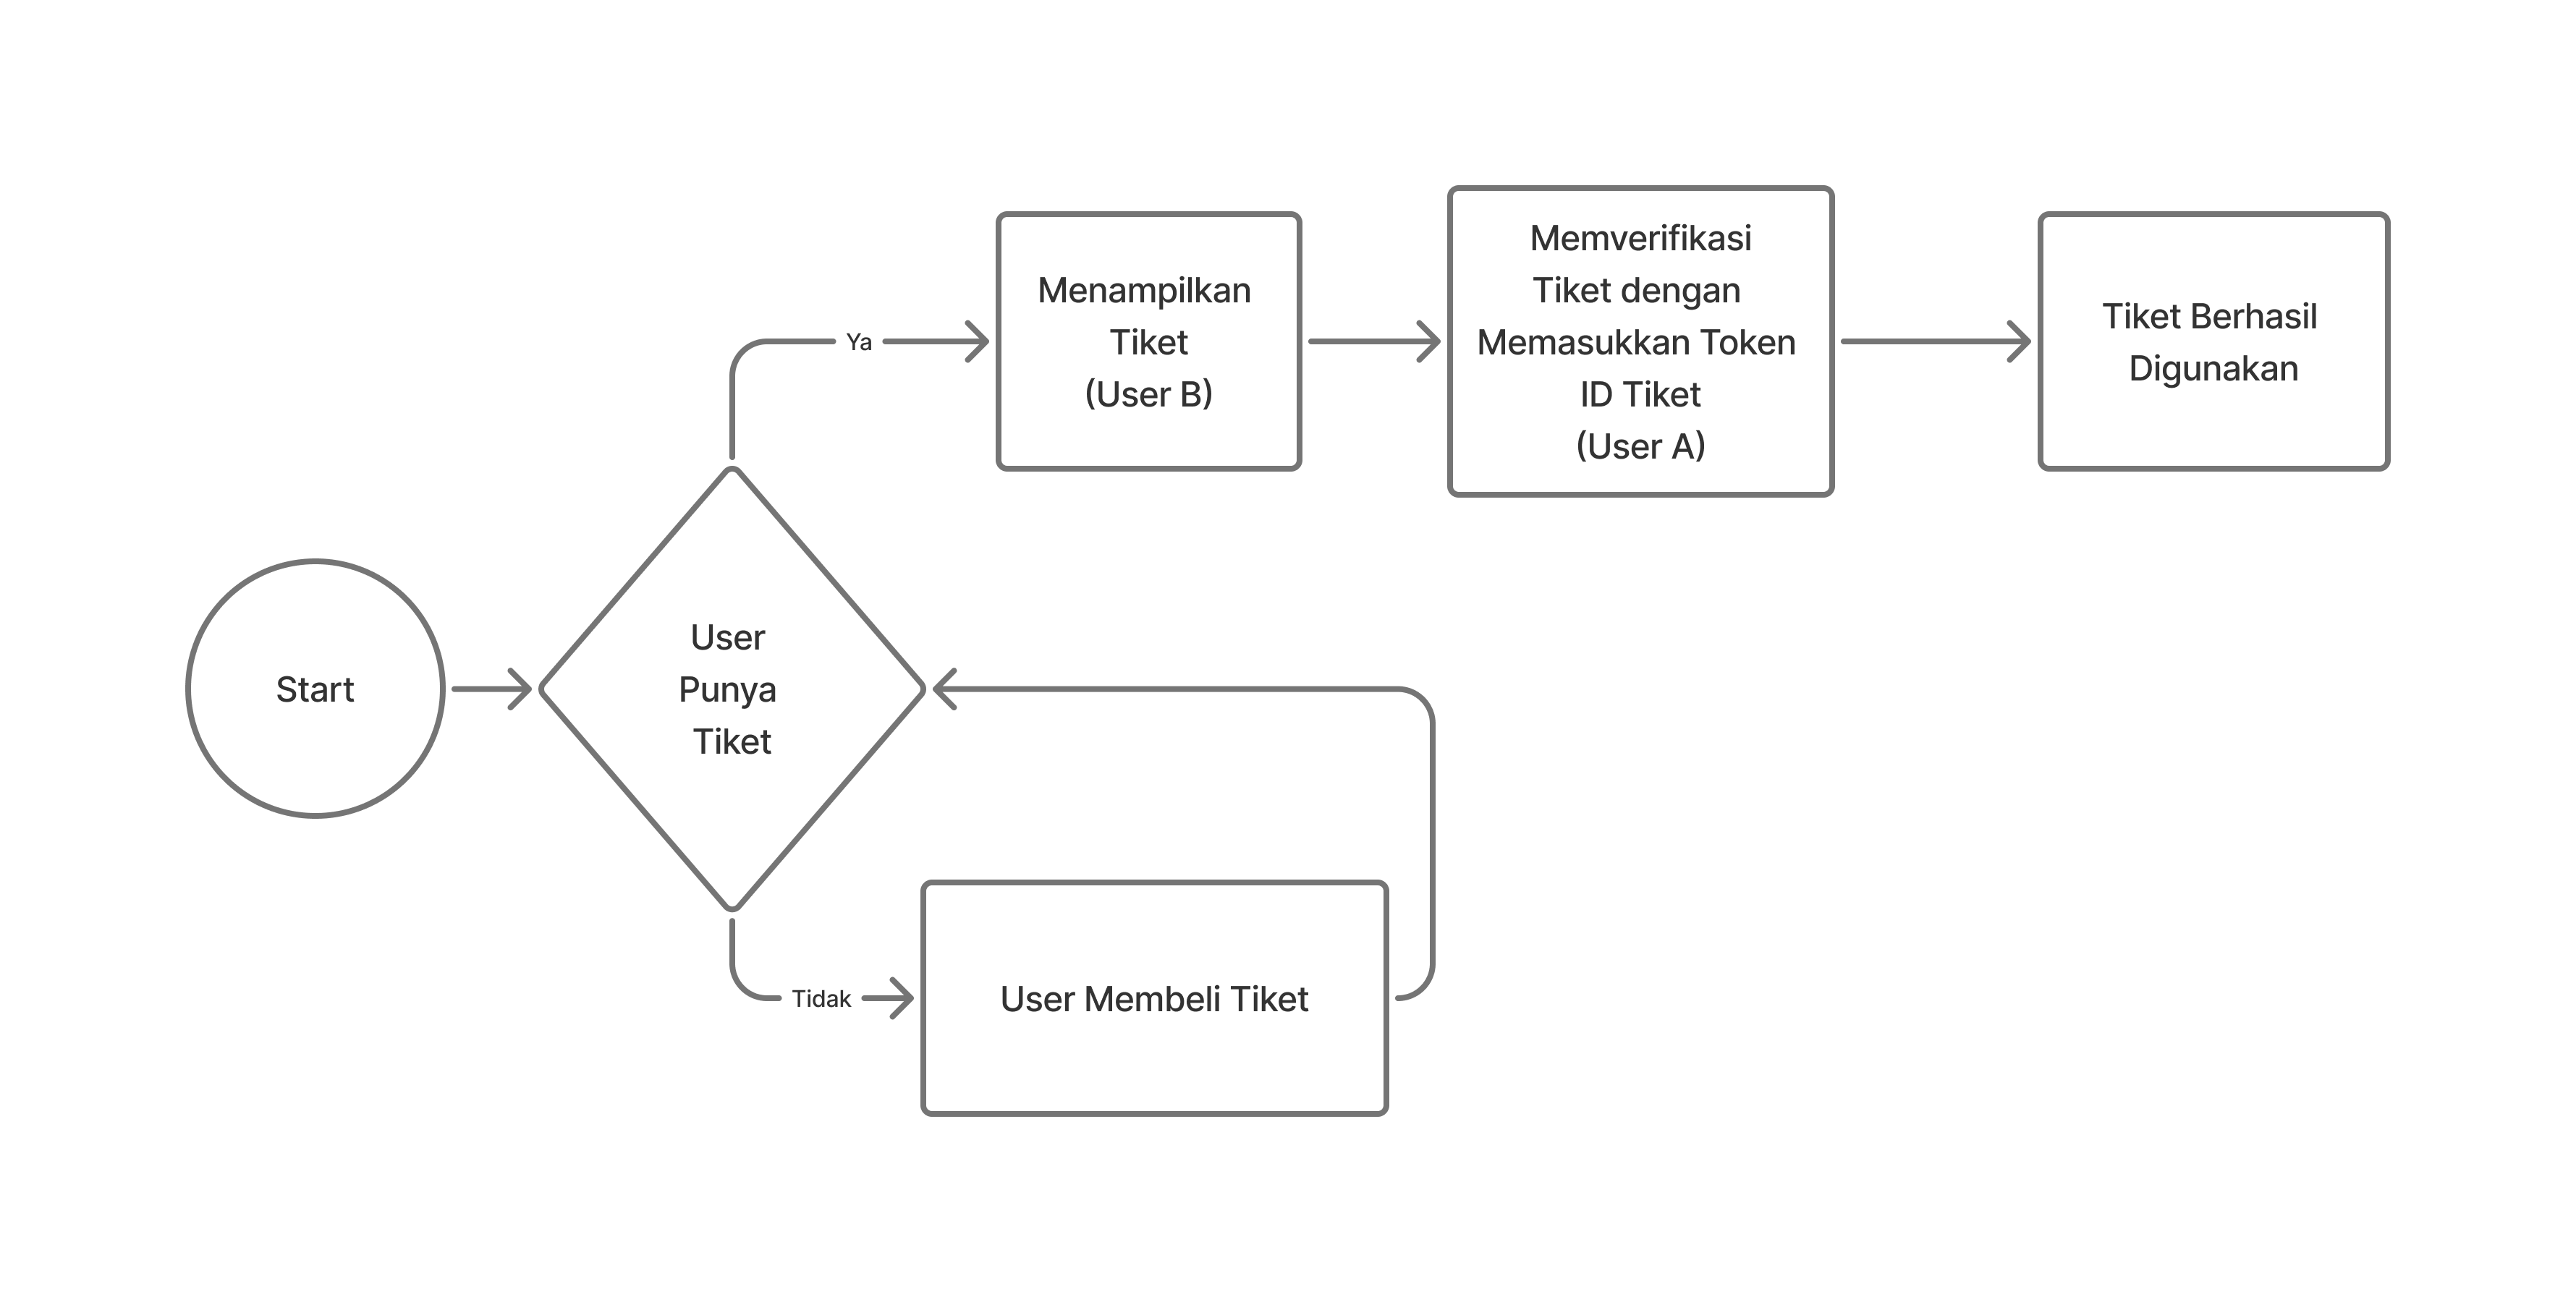
\includegraphics[width=.9\textwidth]{gambar/bab3/Untitled (5).png}
    \caption{Proses Validasi dan Penggunaan Tiket dalam Sistem TicketMarketplace}
    \label{fig:flow-2}
\end{figure}
Gambar \ref{fig:flow-2} menampilkan diagram alur proses yang komprehensif mengenai validasi dan penggunaan tiket dalam sistem \emph{TicketMarketplace} berbasis \emph{blockchain}, mengilustrasikan bagaimana teknologi \emph{NFT (Non-Fungible Token)} diimplementasikan untuk memastikan keaslian dan mencegah penipuan dalam sistem \emph{ticketing} digital. \emph{Flowchart} ini menggambarkan jalur kritis yang harus dilalui oleh pengguna untuk memvalidasi kepemilikan tiket mereka dan menggunakan tiket tersebut untuk mengakses acara, dengan menerapkan proses verifikasi multi-langkah yang memanfaatkan teknologi \emph{blockchain} untuk menyediakan mekanisme validasi yang aman dan anti kerusakan. Proses dimulai dari titik "Start" yang mengarah ke titik keputusan berbentuk berlian berlabel "User Punya Tiket", yang mewakili pemeriksaan otentikasi awal dimana sistem harus memverifikasi apakah pengguna yang mengakses sistem memiliki kepemilikan tiket yang sah untuk acara yang dimaksud. Poin keputusan ini penting karena berfungsi sebagai gerbang yang mencegah akses tidak sah dan memastikan bahwa hanya pemegang tiket sah yang dapat melanjutkan proses validasi. Dalam penerapan sistem tiket berbasis \emph{blockchain}, pemeriksaan ini biasanya melibatkan kueri \emph{smart contract} untuk memverifikasi kepemilikan \emph{NFT} berdasarkan alamat dompet pengguna dan \emph{token ID} yang terkait dengan peristiwa tertentu.

Jika hasil dari verifikasi kepemilikan adalah positif ("Ya"), alur proses
berlanjut ke tahap "Menampilkan Tiket (Pengguna B)", yang menunjukkan bahwa
sistem akan menyajikan tiket digital untuk verifikasi pengguna. Tahap ini
meliputi menampilkan informasi tiket yang komprehensif termasuk detail acara,
penetapan kursi, kode \emph{QR} atau pengidentifikasi unik, dan bukti
kriptografi yang diperlukan untuk langkah validasi selanjutnya. Notasi Pengguna
B menunjukkan bahwa dalam skenario ini, terdapat banyak pihak yang terlibat
dalam proses validasi, dengan Pengguna B berpotensi mewakili pemegang tiket
yang memberikan kredensial untuk verifikasi. Tahap selanjutnya adalah
"Memverifikasi Tiket dengan Memasukkan \emph{Token ID} Tiket (User A)", yang
mewakili mekanisme validasi inti dimana verifikator resmi (User A) melakukan
verifikasi kriptografi untuk mengonfirmasi keaslian tiket. Proses ini
melibatkan memasukkan \emph{Token ID} unik yang terkait dengan tiket \emph{NFT}
ke dalam sistem verifikasi, yang selanjutnya menanyakan \emph{blockchain} untuk
mengonfirmasi bahwa token ada, milik pemilik sah, belum pernah digunakan
sebelumnya, dan valid untuk acara dan jangka waktu tertentu. \emph{Token ID}
berfungsi sebagai sidik jari kriptografi yang secara unik mengidentifikasi
setiap tiket dan tidak dapat dipalsukan atau diduplikasi, memberikan mekanisme
keamanan yang kuat untuk mencegah tiket palsu.

Tahap terakhir dalam jalur validasi berhasil adalah "Tiket Berhasil Digunakan",
yang menunjukkan selesainya proses validasi dan penggunaan tiket berhasil.
Tahap ini biasanya melibatkan penandaan tiket sebagai "digunakan" dalam catatan
\emph{blockchain} untuk mencegah pembelanjaan ganda atau penggunaan kembali,
memperbarui catatan kehadiran acara, dan berpotensi memicu fungsi \emph{smart
    contract} tambahan seperti distribusi pendapatan atau pemrosesan pasca acara.
Setelah tiket ditandai sebagai digunakan, catatan kriptografi pada
\emph{blockchain} memberikan bukti transaksi yang tidak dapat diubah,
menciptakan jejak audit yang dapat diverifikasi oleh penyelenggara acara,
otoritas pengatur, atau pemangku kepentingan lain yang memerlukan verifikasi
transaksi.mJalur alternatif dalam diagram alur menunjukkan skenario dimana
pengguna tidak memiliki tiket yang valid ("Tidak"), mengarah ke proses
"Pengguna Membeli Tiket" yang mengarahkan pengguna yang tidak sah ke saluran
pembelian tiket yang sah. Desain ini memastikan bahwa mekanisme kontrol akses
tidak hanya memverifikasi tiket yang ada tetapi juga menyediakan jalur yang
jelas untuk memperoleh akses yang sah, berpotensi mengurangi gesekan bagi
pengguna yang mungkin telah tiba di titik validasi tanpa kredensial yang tepat
tetapi masih memiliki niat sah untuk menghadiri acara.
\subsection{Desain \emph{Smart Contract}}

\begin{figure}[H]
    \centering
    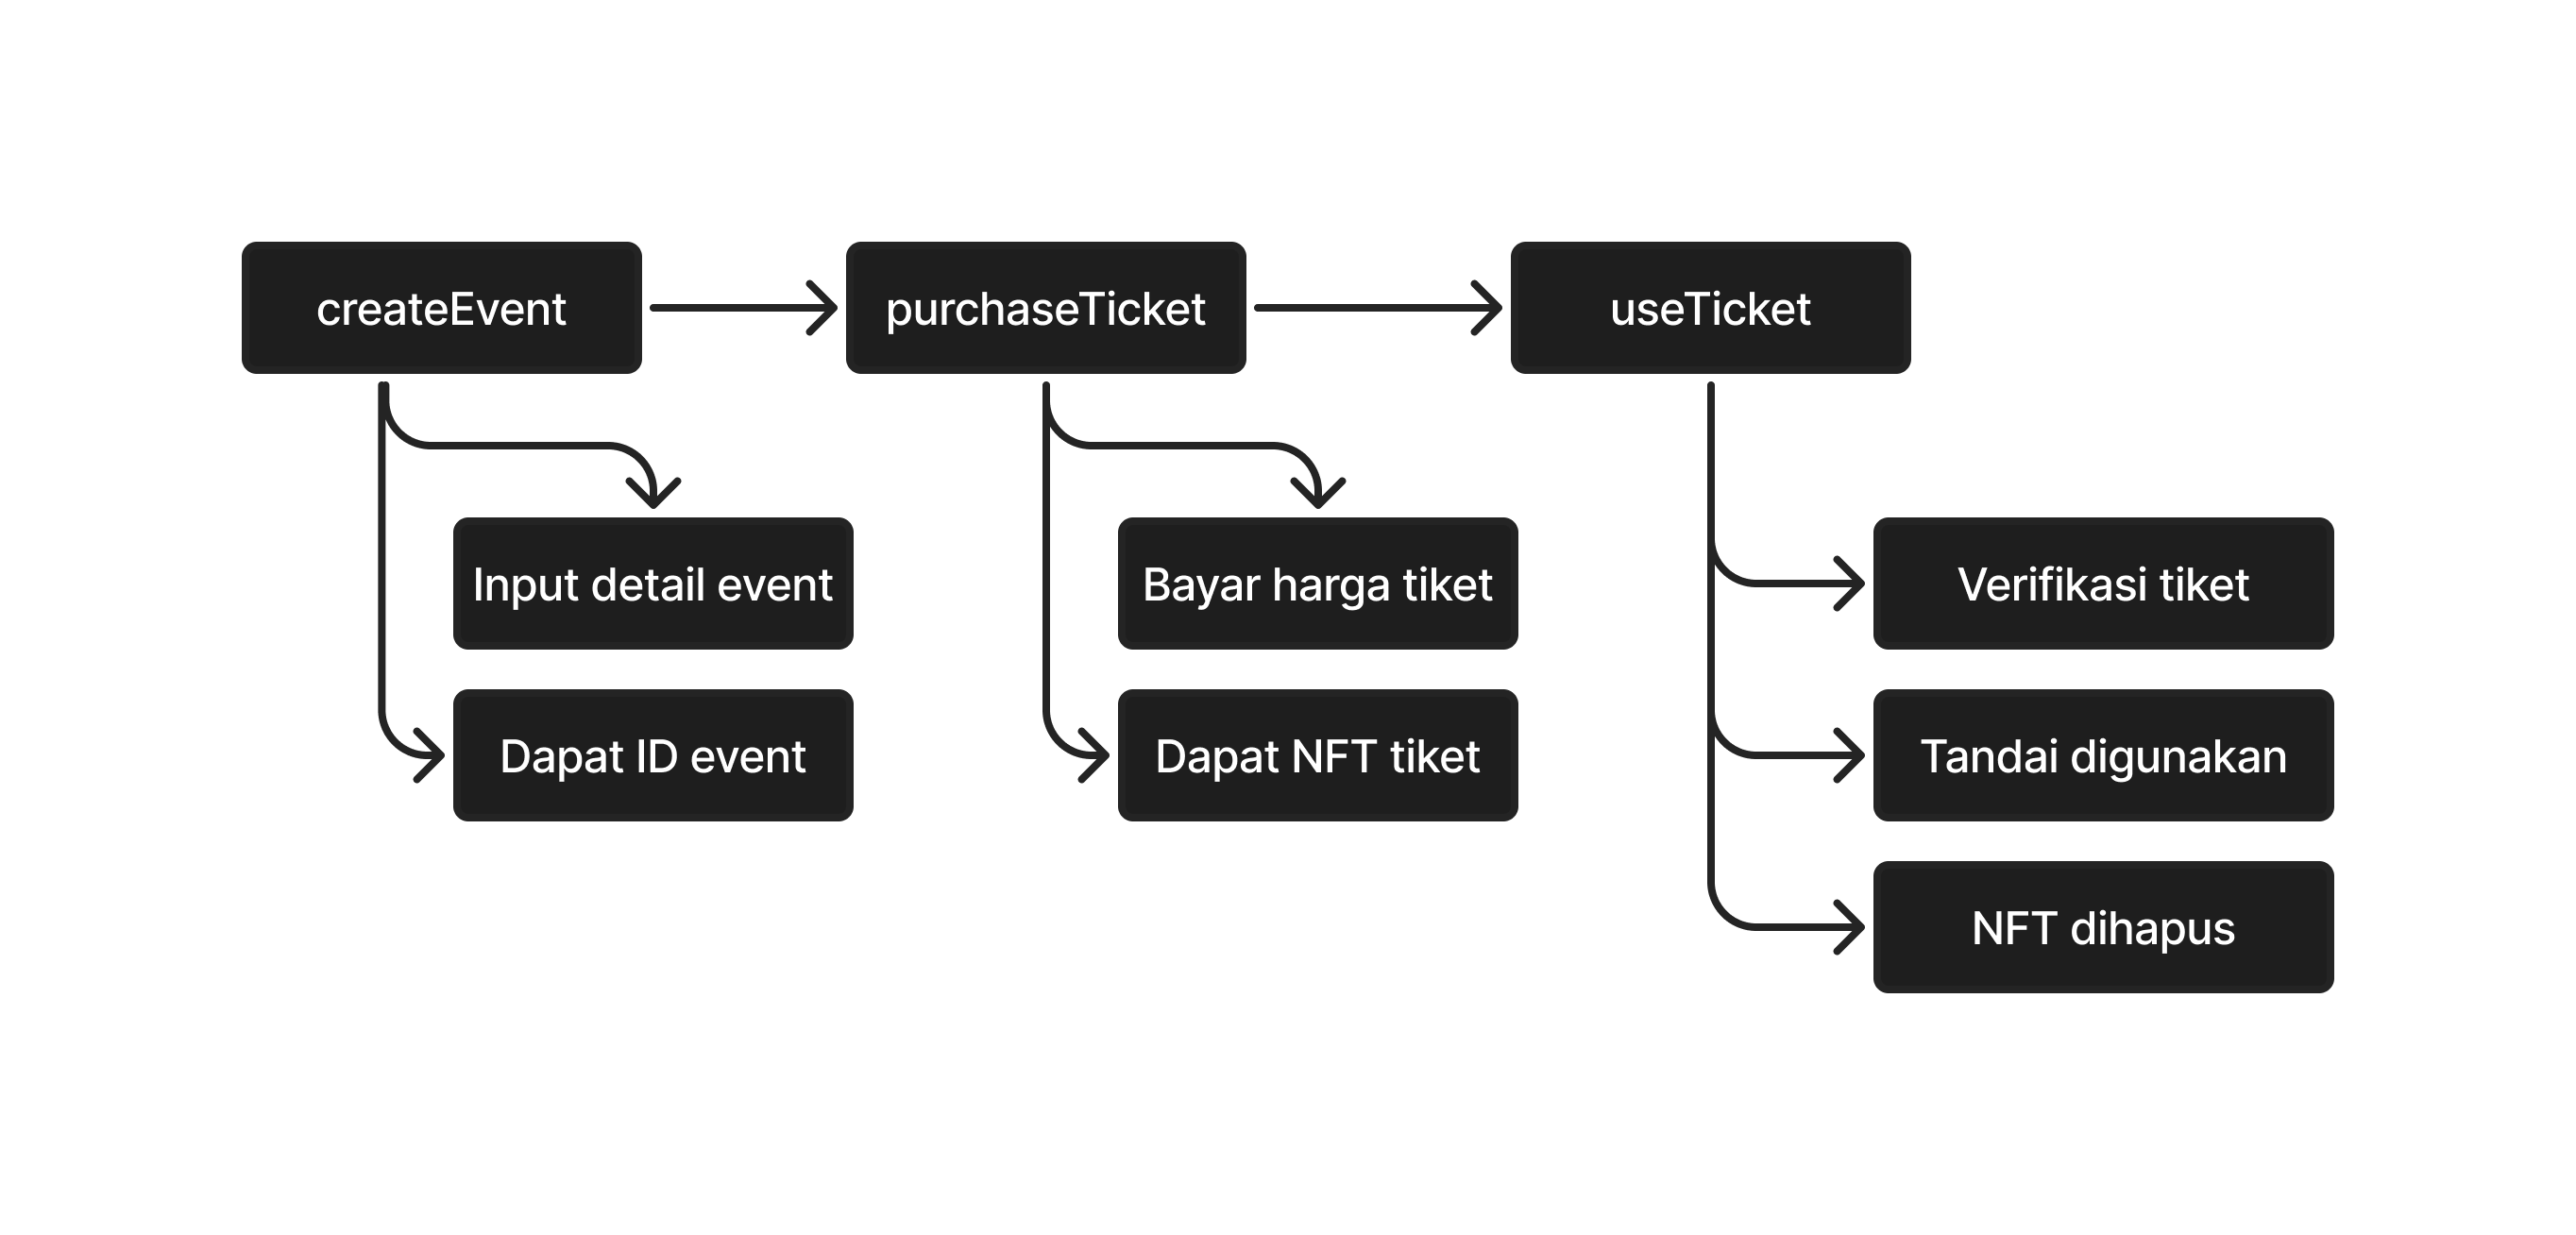
\includegraphics[width=\textwidth]{gambar/bab3/Untitled (3).png}
    \caption{Desain \emph{Smart Contract}}
    \label{fig:desainsmartcontract}
\end{figure}
Sistem marketplace tiket konser berbasis \emph{smart contract} yang dikembangkan memiliki tiga fungsi utama, yaitu createEvent, purchaseTicket, dan useTicket. Ketiga fungsi ini mencerminkan alur bisnis utama dari platform yang dibangun, yakni dari pembuatan acara oleh penyelenggara, pembelian tiket oleh pengguna, hingga proses penggunaan tiket saat konser berlangsung. Setiap fungsi diimplementasikan secara on-chain melalui \emph{smart contract} berbasis Ethereum yang di-deploy pada jaringan Layer-2, dalam hal ini Polygon zkEVM, untuk meningkatkan efisiensi biaya dan performa transaksi.

Fungsi pertama, createEvent, bertugas untuk memungkinkan penyelenggara membuat
event konser baru dengan memasukkan detail yang diperlukan. Informasi yang
dicantumkan antara lain nama event, lokasi, waktu pelaksanaan, jumlah tiket
yang tersedia, dan harga tiket. Data tersebut dikirim sebagai parameter fungsi
dan disimpan secara immutable di dalam \emph{smart contract}. Setelah proses
ini selesai, sistem secara otomatis akan menghasilkan dan mengembalikan sebuah
ID unik sebagai identitas dari event yang baru dibuat. ID ini penting karena
akan digunakan untuk menghubungkan antara event, tiket, dan proses transaksi
pembelian.

Fungsi kedua adalah purchaseTicket, yang menjadi inti dari proses transaksi
antara pengguna dan sistem. Untuk membeli tiket, pengguna harus memilih ID
event yang tersedia, kemudian mengirimkan transaksi dengan menyertakan nilai
pembayaran yang sesuai dengan harga tiket. Setelah transaksi diverifikasi dan
pembayaran berhasil, sistem akan mencetak tiket dalam bentuk Non-Fungible Token
(NFT) kepada alamat wallet pengguna. NFT ini secara otomatis dikaitkan dengan
ID event terkait dan menyimpan informasi metadata tiket yang sebelumnya telah
diunggah ke IPFS. Penggunaan NFT sebagai tiket memberikan jaminan atas
keaslian, transparansi, dan ketidakmungkinan untuk dipalsukan atau digandakan.

Selanjutnya, ketika pengguna menghadiri acara konser, mereka dapat menggunakan
tiket NFT tersebut melalui fungsi useTicket. Fungsi ini hanya dapat dipanggil
oleh pengguna yang merupakan pemilik sah dari NFT tiket. Proses useTicket
terdiri dari tiga tahap utama: pertama adalah verifikasi kepemilikan dan
validitas tiket, kemudian sistem akan menandai tiket tersebut sebagai “sudah
digunakan” agar tidak bisa dipakai kembali, dan terakhir adalah melakukan
proses burn (penghapusan NFT) sebagai langkah akhir untuk menghindari
penyalahgunaan. Semua proses ini tercatat di dalam blockchain, menjadikannya
dapat diaudit dan tidak bisa dimanipulasi.

Dengan implementasi tiga fungsi utama ini, sistem menyediakan alur kerja yang
lengkap dan aman mulai dari hulu hingga hilir. Fungsi createEvent menjamin
bahwa hanya penyelenggara yang dapat menambahkan acara; purchaseTicket menjamin
bahwa tiket hanya diberikan kepada pembeli yang sah; dan useTicket memastikan
bahwa tiket hanya dapat digunakan satu kali oleh pemiliknya. Kombinasi dari
\emph{smart contract}, NFT, dan teknologi Layer-2 ini tidak hanya memberikan
efisiensi dan keamanan, tetapi juga transparansi tinggi dalam seluruh proses
transaksi dan validasi tiket konser.

\subsection{Desain Antarmuka Pengguna}
\begin{figure}[H]
    \centering
    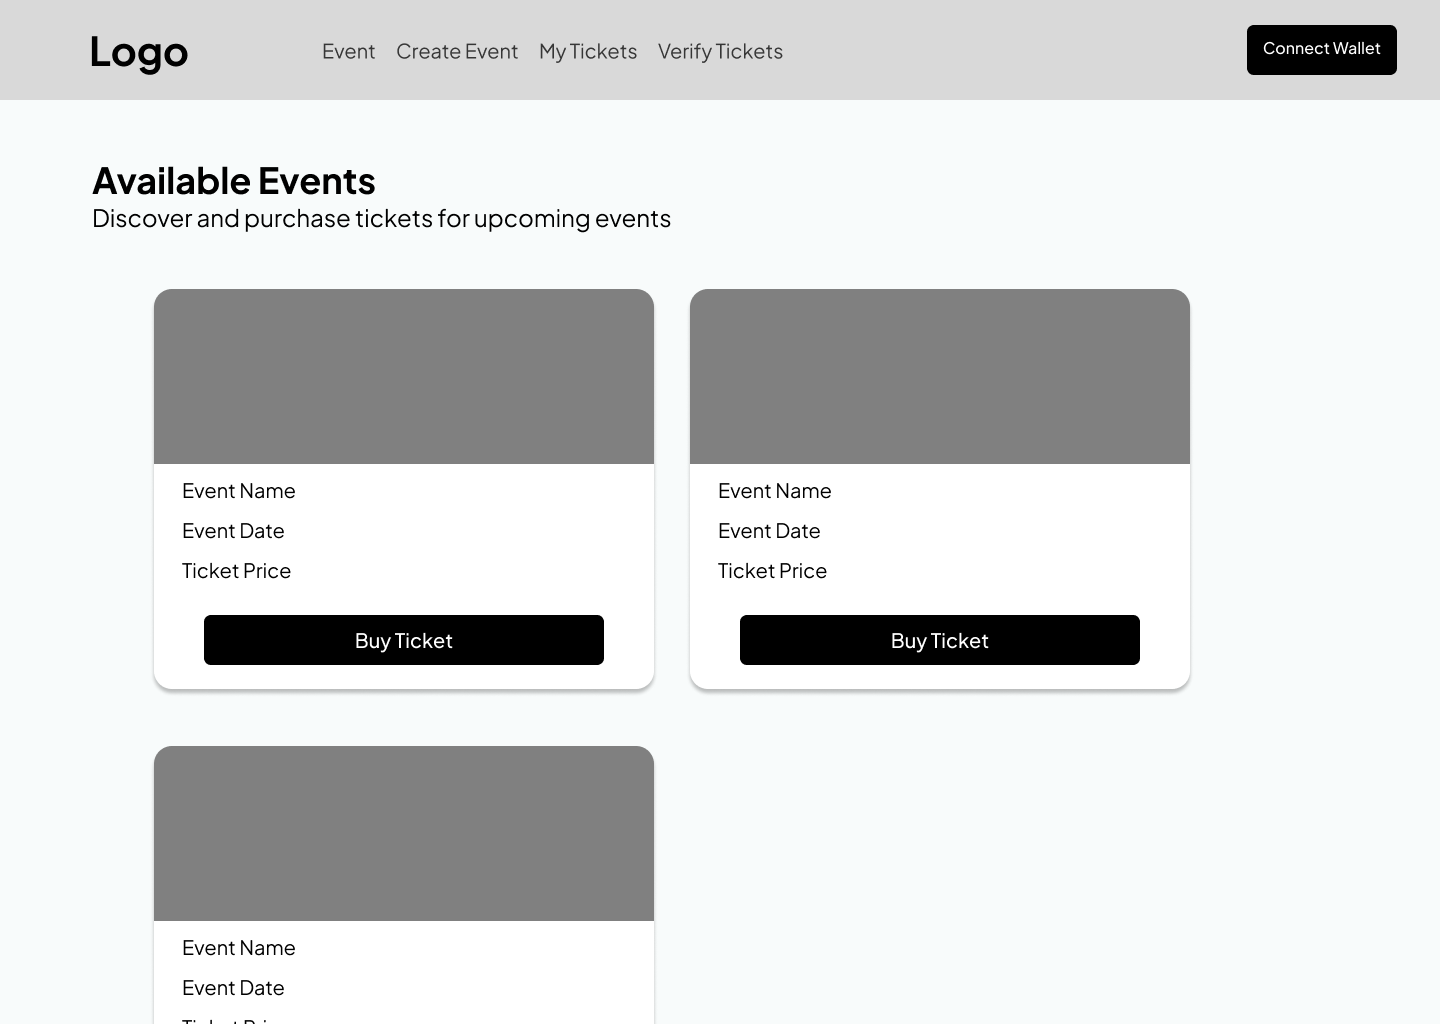
\includegraphics[width=.9\textwidth]{gambar/bab3/Wireframe - 1.png}
    \caption{Wireframe halaman utama}
    \label{fig:wireframe-1}
\end{figure}

Gambar \ref{fig:wireframe-1} menunjukkan halaman "Available Events" yang
berfungsi sebagai pasar utama dimana calon pelanggan dapat menemukan dan
membeli tiket untuk acara mendatang. Antarmuka ini mengimplementasikan tata
letak berbasis kartu yang familiar dan ramah pengguna, memungkinkan penelusuran
yang mudah melalui acara yang tersedia dengan hierarki visual yang jelas.
Setiap kartu acara menampilkan informasi penting yang dibutuhkan pelanggan
untuk mengambil keputusan, termasuk nama acara, tanggal, dan harga tiket,
dengan tombol "Beli Tiket" yang menonjol yang memfasilitasi tindakan pembelian
segera. Desain menggunakan gambar placeholder dalam format persegi panjang yang
konsisten, menunjukkan bahwa dalam implementasi, setiap acara akan ditampilkan
dengan konten visual yang menarik seperti foto artis, gambar venue, atau grafik
promosi yang meningkatkan keterlibatan pengguna. Sistem grid tata letak
memungkinkan pemanfaatan ruang dan skalabilitas yang efisien untuk menampilkan
peristiwa dalam jumlah besar tanpa membebani pengguna. Tombol ajakan bertindak
yang ditampilkan secara jelas dengan gaya yang konsisten di seluruh kartu
memastikan proses pembelian dapat dimulai dengan gesekan minimal. Penerapan
fungsi pasar sangat penting untuk menciptakan ekosistem yang dinamis dimana
penyelenggara acara dapat menjangkau khalayak yang lebih luas sementara
pelanggan memiliki akses ke beragam pilihan hiburan dengan sistem tiket
tepercaya dan terverifikasi blockchain.

\begin{figure}[H]
    \centering
    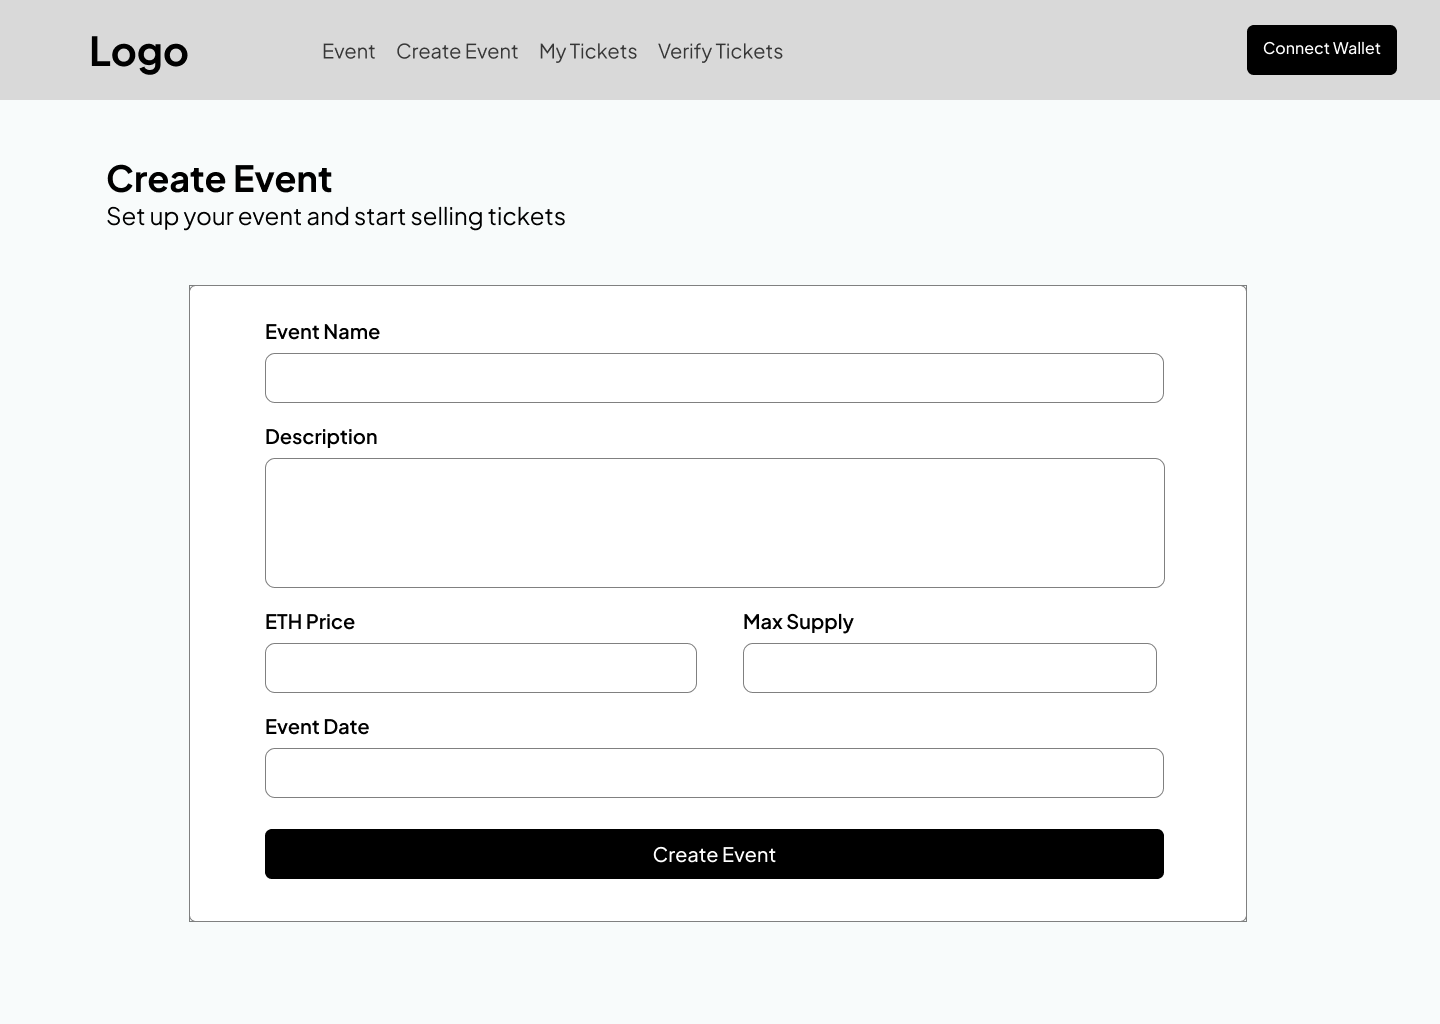
\includegraphics[width=.9\textwidth]{gambar/bab3/Wireframe - 2.png}
    \caption{Wireframe membuat event}
    \label{fig:wireframe-2}
\end{figure}
Gambar \ref{fig:wireframe-2} menampilkan halaman "Create Event" yang merupakan antarmuka bentuk komprehensif yang dirancang untuk penyelenggara acara dalam menyiapkan acara baru dan meluncurkan penjualan tiket melalui platform. Antarmuka ini mengimplementasikan desain bersih dan berbasis formulir yang memandu penyelenggara melalui langkah-langkah penting dalam proses pembuatan acara dengan alur logis dan label bidang yang jelas. Struktur formulir menunjukkan pendekatan sistematis dalam pengumpulan data, dimulai dengan informasi peristiwa dasar seperti "Nama Event" dan "Deskripsi", diikuti oleh parameter komersial seperti "Harga ETH" dan "Pasokan Maksimum", dan diakhiri dengan spesifikasi temporal melalui kolom "Tanggal Peristiwa".
Pemisahan antara berbagai jenis bidang - input teks untuk informasi deskriptif, input numerik untuk parameter keuangan dan kapasitas, dan pemilih tanggal untuk penjadwalan - menunjukkan desain UX yang bijaksana yang mengakomodasi berbagai jenis entri data dengan mekanisme input yang sesuai. Area teks deskripsi yang besar memungkinkan penyelenggara untuk memberikan rincian acara yang komprehensif yang dapat membantu pelanggan membuat keputusan pembelian yang tepat, sementara tata letak berdampingan untuk bidang "Harga ETH" dan "Pasokan Maks" memungkinkan perbandingan dan penyesuaian yang mudah dari parameter komersial utama. Tombol tengah "Buat Acara" yang ditampilkan secara jelas dengan gaya yang konsisten memberikan ajakan bertindak yang jelas untuk menyelesaikan proses pembuatan acara.
Antarmuka ini mewakili komponen penting dalam ekosistem platform karena memungkinkan demokratisasi dari penyelenggaraan acara, memungkinkan penyelenggara kecil atau seniman independen untuk mengakses infrastruktur tiket berbasis blockchain tanpa memerlukan pengetahuan teknis yang luas atau investasi awal yang signifikan. Integrasi dengan fungsionalitas \emph{smart contract} memastikan bahwa semua peristiwa yang dibuat melalui antarmuka ini secara otomatis mendapatkan manfaat dari keamanan blockchain, transparansi, dan kemampuan pemrosesan pembayaran otomatis yang melekat dalam sistem pasar terdesentralisasi.

\begin{figure}[H]
    \centering
    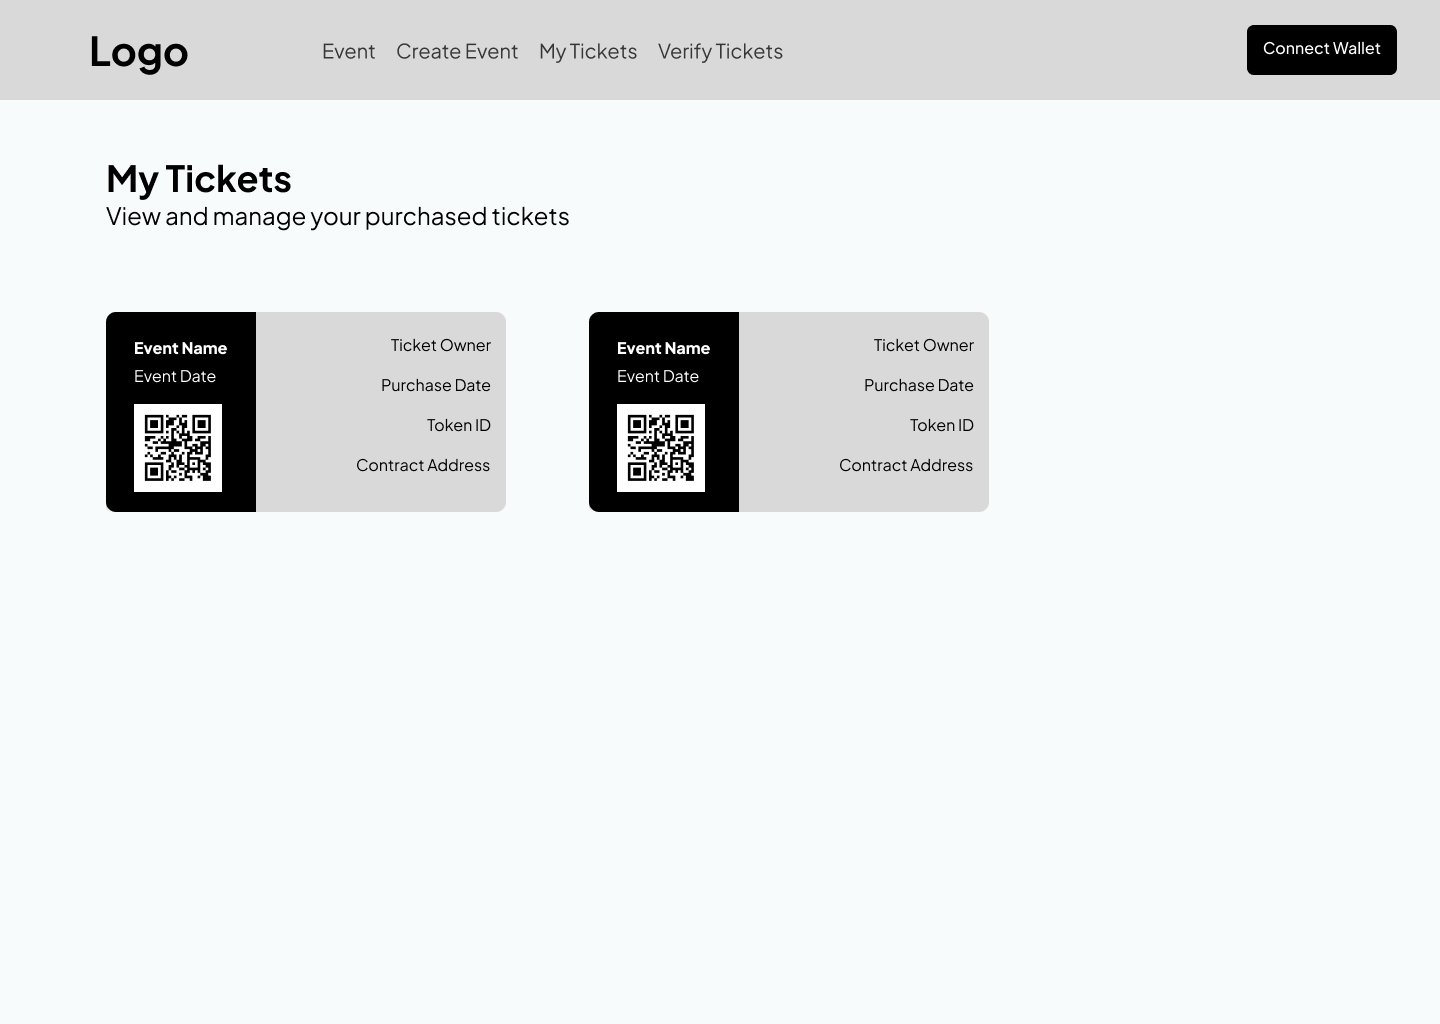
\includegraphics[width=.9\textwidth]{gambar/bab3/Wireframe - 3.png}
    \caption{Wireframe tiket yang dimiliki}
    \label{fig:wireframe-3}
\end{figure}
Gambar \ref{fig:wireframe-3} menampilkan halaman "My Tickets" yang merupakan dashboard personal untuk pengguna dalam mengelola koleksi tiket digital yang telah mereka beli melalui platform Ticket Marketplace. Antarmuka ini dirancang dengan pendekatan user-centric yang memungkinkan pengguna untuk dengan mudah mengakses dan mengelola seluruh tiket NFT yang dimiliki dalam satu lokasi keinginan.
Halaman ini menampilkan dua contoh tiket dalam format card yang menunjukkan informasi penting seperti nama event, tanggal event, pemilik tiket, tanggal pembelian, Token ID yang unik, dan alamat kontrak. Setiap tiket dilengkapi dengan QR code yang berfungsi sebagai mekanisme verifikasi digital, memungkinkan validasi cepat dan aman di lokasi acara tanpa memerlukan proses manual yang memakan waktu. Desain visual menggunakan kontras warna yang jelas antara background hitam dan abu-abu, memberikan informasi hierarki yang memudahkan pengguna dalam memindai informasi dengan cepat. Implementasi kode QR pada setiap tiket merepresentasikan inovasi dalam tiket digital dimana keaslian dan kepemilikan dapat dikonfigurasi secara real-time melalui teknologi blockchain, menghilangkan risiko tiket palsu yang biasa ditemukan dalam sistem tiket tradisional.
\begin{figure}[H]
    \centering
    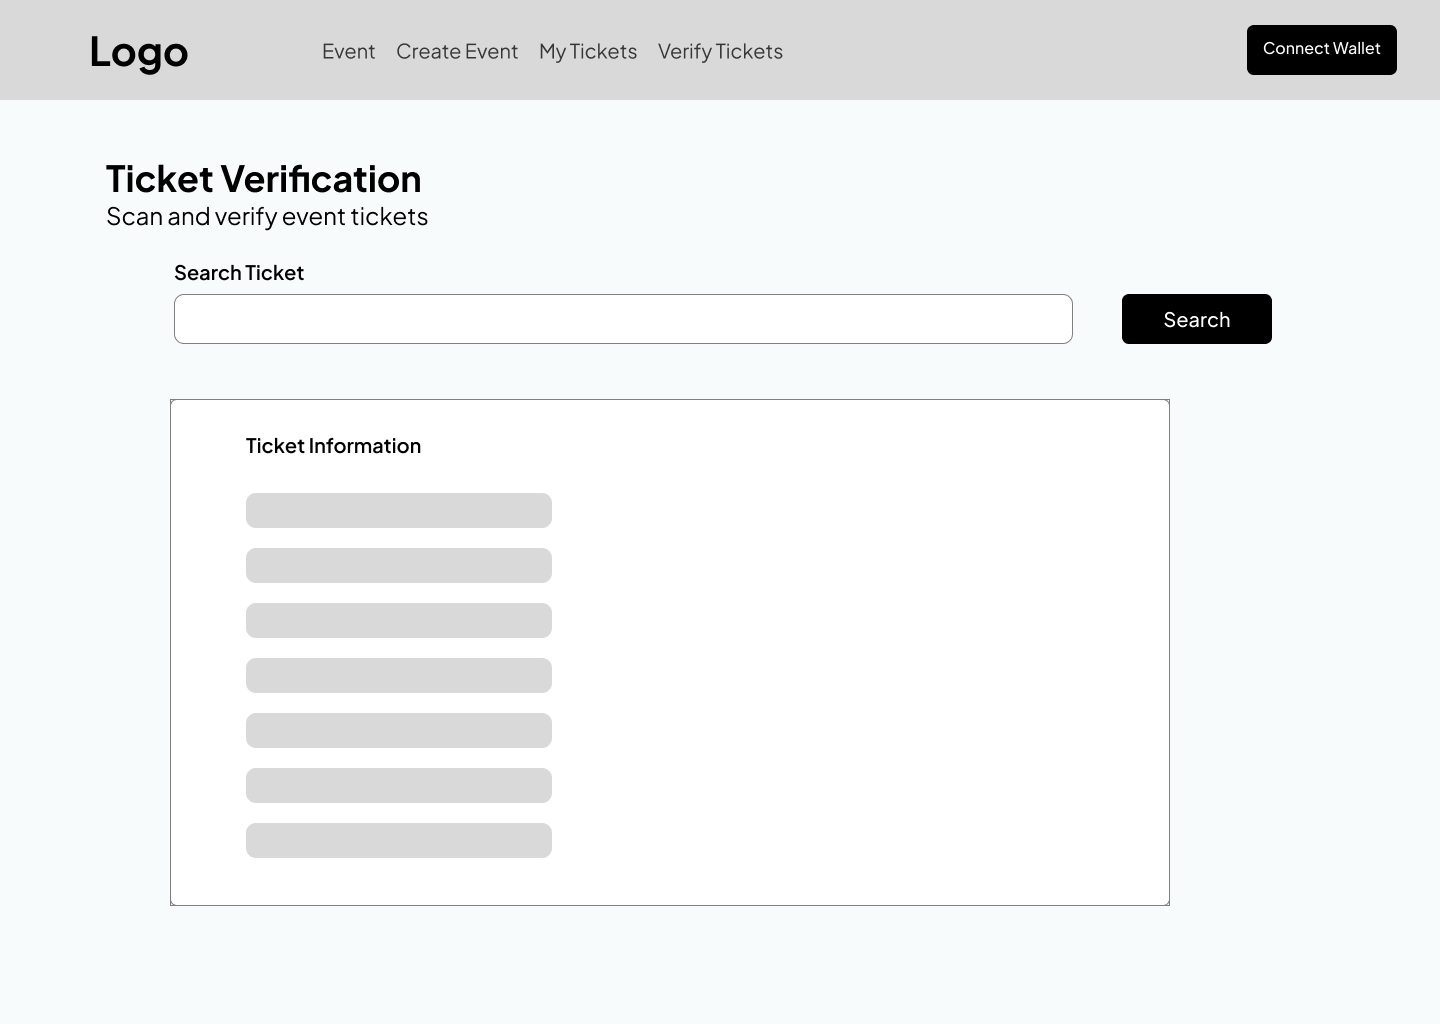
\includegraphics[width=.9\textwidth]{gambar/bab3/Wireframe - 4.png}
    \caption{Wireframe penggunaan tiket}
    \label{fig:wireframe-4}
\end{figure}
Gambar \ref{fig:wireframe-4} menampilkan halaman "Verifikasi Tiket" yang merupakan alat penting untuk staf acara dan personel keamanan dalam melakukan validasi tiket di pintu masuk venue. Antarmuka ini dirancang dengan fokus pada fungsionalitas dan kemudahan penggunaan, mengingat bahwa pengguna utama adalah staf yang mungkin perlu melakukan verifikasi ratusan tiket dalam jangka waktu singkat. Fungsi pencarian yang menonjol dengan kolom input yang besar dan tombol "Search" yang terlihat jelas memungkinkan pencarian cepat untuk tiket tertentu menggunakan berbagai pengidentifikasi seperti Token ID, hash transaksi, atau alamat dompet.
Bagian "Informasi Tiket" yang ditampilkan sebagai placeholder dengan beberapa bilah abu-abu menunjukkan bahwa setelah pencarian berhasil, halaman ini akan menampilkan detail lengkap tentang tiket yang dicari, termasuk status validasi, detail acara, riwayat kepemilikan, dan bukti otentikasi. Desain antarmuka yang minimalis ini sengaja mengurangi gangguan dan memungkinkan staf untuk fokus pada tugas verifikasi inti tanpa kerumitan yang tidak perlu. Integrasi dengan infrastruktur blockchain memungkinkan verifikasi real-time terhadap keaslian tiket, memastikan bahwa hanya pemegang tiket sah yang dapat memperoleh akses ke acara. Sistem ini juga dapat melacak status penggunaan untuk mencegah skenario entri ganda dan menyimpan catatan kehadiran yang akurat untuk penyelenggara acara.

Antarmuka pengguna (frontend) untuk marketplace tiket konser berbasis smart
contract dirancang sebagai aplikasi Web3 yang menyeluruh, berfungsi sebagai
jembatan yang mulus antara pengalaman pengguna web tradisional dan teknologi
blockchain, sekaligus memungkinkan interaksi langsung dan aman dengan smart
contract yang telah diunggah ke jaringan Polygon zkEVM. Struktur antarmuka ini
mengikuti praktik pengembangan web modern dengan penekanan pada pengoptimalan
pengalaman pengguna, efisiensi kinerja, dan pertismbangan keamanan yang sangat
penting dalam aplikasi keuangan yang menangani transaksi kripto dan aset
digital berharga seperti tiket NFT. Proses pengembangan dimulai dengan
inisialisasi proyek menggunakan framework Next.js versi 15, yang menyediakan
kemampuan server-side rendering, pemisahan kode otomatis untuk mempercepat
pemuatan halaman, serta fitur bawaan seperti pengoptimalan gambar, pemuatan
huruf, dan sistem routing yang tangguh untuk mendukung halaman-halaman dinamis
baik untuk acara maupun pengguna.

Struktur App Router dari Next.js memungkinkan pemetaan berdasarkan struktur
berkas, dukungan untuk tata letak bertingkat (nested layout), status pemuatan,
serta penanganan kesalahan secara terpisah—yang sangat penting dalam menangani
status operasi blockchain dan gangguan konektivitas jaringan yang umum dalam
aplikasi Web3. Integrasi TypeScript memberikan pengecekan tipe secara statis
yang meningkatkan pengalaman pengembang dan mengurangi kesalahan saat aplikasi
dijalankan—khususnya penting dalam pengembangan Web3 di mana interaksi dengan
\emph{smart contract} memerlukan tipe parameter dan nilai keluaran yang tepat.
Definisi tipe khusus disiapkan untuk entitas aplikasi seperti Event dan Ticket,
sementara tipe umum mencakup alamat dompet, objek transaksi, log peristiwa
(event log), dan antarmuka kontrak (contract interface). Libary utama untuk
interaksi dengan blockchain menggunakan ethers.js versi 6, yang menyediakan
seperangkat alat untuk memanggil metode \emph{smart contract}, mengelola
transaksi, mendengarkan peristiwa, dan mengintegrasikan dompet pengguna.
Penyedia (provider) dari ethers.js mendukung koneksi ke berbagai titik RPC
(Remote Procedure Call) dengan kemampuan pemulihan otomatis jika terjadi
gangguan jaringan atau layanan.

Kontrak dibangun menggunakan contract factory dan tipe-tipe yang dihasilkan
dari berkas ABI (Application Binary Interface), memungkinkan interaksi aman dan
terstruktur dengan dukungan fitur IntelliSense untuk metode dan peristiwa dalam
kontrak. Setelah infrastruktur dasar dikonfigurasi, implementasi koneksi dompet
mencakup pengelolaan status koneksi, penanganan perubahan akun, validasi
jaringan untuk memastikan pengguna terhubung ke jari-ngan yang benar (misalnya
testnet Cardona untuk pengembangan atau jaringan produksi untuk peluncuran),
serta mekanisme penyambungan ulang otomatis agar sesi pengguna tetap bertahan
meski halaman dimuat ulang atau browser ditutup. Permintaan untuk mengganti
jaringan ditampilkan kepada pengguna ketika mereka terhubung ke jaringan yang
tidak sesuai, dengan petunjuk yang jelas serta dukungan penambahan jaringan
baru secara otomatis jika belum tersedia di dompet pengguna.

\subsection{Pengembangan \emph{Smart Contract}}
\emph{Smart contract} dikembangkan menggunakan Solidity versi 0.8.28, bahasa
pemrograman utama untuk blockchain Ethereum dan Polygon zkEVM yang menyediakan
sintaksis yang familier bagi pengembang dengan latar belakang JavaScript atau
C++. Solidity merupakan bahasa pemrograman yang diketik secara statis secara
spesifik dirancang untuk mengembangkan \emph{smart contract} yang berjalan pada
Ethereum Virtual Machine (EVM), dengan fitur-fitur seperti warisan,
perpustakaan, dan tipe kompleks yang ditentukan pengguna yang memungkinkan
pengembangan aplikasi blockchain yang canggih dan aman. Versi 0.8.28 yang
digunakan dalam penelitian ini memberikan perlindungan overflow/underflow
bawaan, penanganan kesalahan yang ditingkatkan mekanisme, dan peningkatan fitur
optimalisasi gas yang penting untuk operasi hemat biaya pada jaringan Layer-2
seperti Polygon zkEVM.Untuk pengembangan, pengujian, dan penerapan, Hardhat
digunakan sebagai yang utama kerangka pengembangan yang memungkinkan kompilasi,
pengujian, penerapan cerdas kontrak, dan kemampuan debugging yang komprehensif.
Hardhat menyediakan ekosistem lengkap yang terintegrasi dengan dukungan untuk
skrip tingkat lanjut menggunakan JavaScript/TypeScript, pengujian otomatis
menggunakan tes Mocha framework dan perpustakaan pernyataan Chai, serta alat
debugging yang kuat termasuk fungsionalitas console.log dalam \emph{smart contract},
pelacakan tumpukan hingga gagal transaksi, dan analisis penggunaan gas.
Framework ini juga menyediakan built-in lingkungan blockchain lokal melalui
Hardhat Network yang memungkinkan cepat siklus pengembangan dengan penambangan
instan, harga gas yang dapat dikonfigurasi, dan detail transaksi logging untuk
skenario pengujian yang komprehensif.

Konfigurasi Hardhat memungkinkan penerapan multi-jaringan dengan mudah beralih
antara lingkungan pengembangan, testnet, dan mainnet melalui single file
konfigurasi yang men-definisikan parameter jaringan, manajemen akun, dan
strategi penerapan. Ekosistem plugin yang mencakup integrasi luas dengan alat
seperti Etherscan untuk verifikasi kontrak, OpenZeppelin untuk audit keamanan,
pelaporan gas untuk analisis biaya, dan alat cakupan untuk pengujian pengukuran
kelengkapan. Sistem Tugas Hardhat memungkinkan pembuatan skrip khusus untuk
alur kerja otomatis seperti penerapan kontrak, data penyemaian, dan operasi
administratif yang dapat dijalankan dengan konsisten parameter di lingkungan
yang berbeda. Alur kerja pengembangan menggunakan Hardhat meliputi beberapa
tahapan yang sistematis: kontrak pengembangan dengan pemeriksaan kompilasi
waktu nyata, pengujian unit komprehensif menggunakan tes perlengkapan dan
kontrak tiruan, pengujian integrasi dengan pengguna simulasi interaksi,
analisis optimasi gas untuk mengidentifikasi hambatan biaya, dan skrip
penerapan otomatis yang memastikan penerapan yang konsisten di banyak tempat
jaringan. Hardhat Console menyediakan lingkungan JavaScript interaktif yang
memungkinkan interaksi real-time dengan kontrak yang diterapkan, berguna untuk
debugging, kueri data, dan operasi administratif tanpa perlu menulis skrip
terpisah. Kerangka pengujian yang kuat mencakup pengujian unit untuk fungsi
kontrak individual, pengujian integrasi untuk multi-kontrak interaksi, stress
test untuk skenario volume tinggi, dan edge case test untuk kerentanan
keamanan. Mocha test runner memberikan tes terstruktur organisasi dengan
mendeskripsikan blok, sebelum/sesudah kait untuk pengaturan/pembongkaran
operasi, dan pelaporan pengujian terperinci dengan metrik penggunaan gas. Chai
perpustakaan pernyataan memungkinkan pernyataan pengujian ekspresif dengan
kustom pencocokan untuk operasi khusus blockchain seperti pemeriksaan emisi
peristiwa, kembalikan validasi alasan, dan verifikasi perubahan status.
Arsitektur plugin Hardhat memungkinkan perluasan melalui plugin yang
dikembangkan komunitas tambahkan fungsionalitas seperti pemeriksaan ukuran
kontrak otomatis untuk batas penerapan, integrasi analisis keamanan dengan alat
seperas Slither atau MythX, dan pemantauan kinerja untuk metrik eksekusi
transaksi. Plugin Hardhat Verify memungkinkan verifikasi kode sumber otomatis
pada penjelajah blok, penting untuk transparansi dan kepercayaan pengguna dalam
penerapan produksi. Plugin reporter gas memberikan analisis biaya secara rinci
operasi untuk setiap panggilan fungsi, memungkinkan keputusan optimasi
berdasarkan pola penggunaan sebenarnya. Manajemen konfigurasi melalui File
hardhat.config.js memungkinkan pengaturan canggih untuk berbeda skenario
penerapan, termasuk harga gas spesifik jaringan, manajemen akun dengan
integrasi dompet perangkat keras, dan kontrak khusus lingkungan parameter.
Pengaturan kompiler dapat dikonfigurasi untuk tingkat optimasi yang berbeda,
targetkan versi EVM untuk kompatibilitas yang berbeda jaringan, dan pilihan
keluaran untuk menghasilkan kompilasi yang komprehensif artefak. Konfigurasi
jaringan mendukung beberapa penyedia RPC dengan failover otomatis, strategi
estimasi gas khusus, dan batas waktu konfigurasi untuk interaksi jaringan yang
andal.
\begin{figure}[H]
    \centering
    \begin{subfigure}[b]{0.48\textwidth}
        \centering
        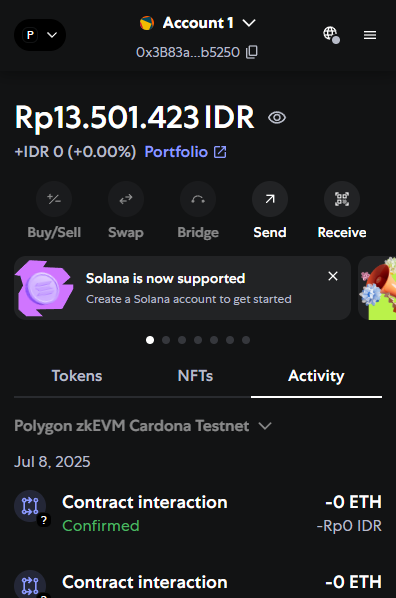
\includegraphics[width=\textwidth]{gambar/bab3/Screenshot 2025-07-08 222752.png}
        \caption{Akun Metamask Seller.}
        \label{fig:akunadmin}
    \end{subfigure}
    \hfill
    \begin{subfigure}[b]{0.48\textwidth}
        \centering
        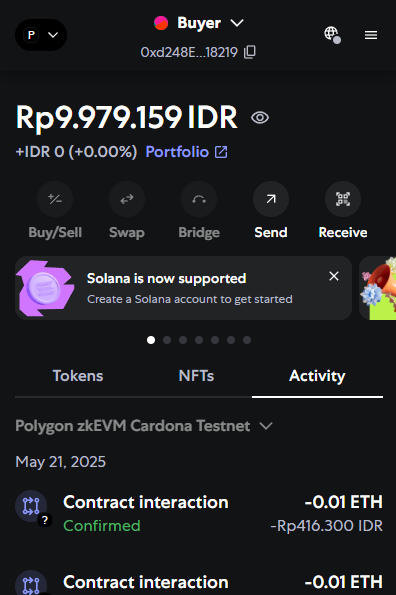
\includegraphics[width=\textwidth]{gambar/bab3/Screenshot 2025-07-08 222807.png}
        \caption{Akun Metamask Pembeli.}
        \label{fig:akunpembeli}
    \end{subfigure}
    \caption{Tampilan Akun Metamask Penjual dan Pembeli}
    \label{fig:akunmetamask}
\end{figure}

\subsection{Perilisan \emph{Smart Contract} ke Testnet} Tahap persiapan pengembangan lingkungan merupakan fondasi penting
yang menentukan keberhasilan seluruh proses penerapan \emph{smart contract}.
Kerangka kerja Hardhat dipilih sebagai lingkungan pengembangan utama karena
ekosistem perkakas komprehensif yang mencakup kemampuan kompilasi, pengujian,
debugging, dan penerapan dalam satu platform terintegrasi. Instalasi Node.js
dengan versi LTS terbaru memastikan kompatibilitas dengan fitur terbaru dan
pembaruan keamanan, sekaligus memberikan landasan yang stabil untuk dependensi
pengembangan. Integrasi TypeScript dikonfigurasi untuk memberikan keamanan tipe
yang penting dalam pengembangan \emph{smart contract}, dimana kesalahan tipe
dapat mengakibatkan kerentanan kritis atau perilaku tak terduga dalam
lingkungan produksi. Pustaka kontrak OpenZeppelin dijadikan landasan untuk
menerapkan pola keamanan standar industri dan menguji implementasi fungsi
\emph{smart contract} umum, secara signifikan mengurangi risiko pengembangan
dan mening-katkan kualitas kode. Konfigurasi variabel lingkungan menggunakan
paket dotenv memastikan informasi sensitif seperti kunci pribadi, titik akhir
API, dan parameter konfigurasi tidak terekspos dalam sistem kontrol versi,
menjaga praktik terbaik keamanan sepanjang siklus hidup pengembangan.

Konfigurasi infrastruktur jaringan merupakan tahap penting yang memastikan
konektivitas yang andal ke jaringan blockchain target dan parameter eksekusi
transaksi yang optimal. Pengaturan titik akhir RPC untuk Ethereum Sepolia
testnet dilakukan melalui integrasi beberapa penyedia termasuk Infura, Alchemy,
dan titik akhir publik untuk memastikan ketersediaan tinggi dan toleransi
kesalahan. Konfigurasi Polygon zkEVM Cardona testnet memerlukan perhatian
khusus terhadap karakteristik unik dari proses verifikasi bukti tanpa
pengetahuan, dengan pengaturan waktu habis yang disesuaikan untuk mengakomodasi
waktu pemrosesan lebih lama yang melekat dalam arsitektur zkEVM. Integrasi
testnet Polygon PoS Amoy dikonfigurasi dengan optimasi untuk karakteristik
throughput tinggi dan ekspektasi latensi lebih rendah yang khas dari solusi
lapisan-2 yang matang. Implementasi penyedia RPC cadangan menggunakan mekanisme
failover otomatis yang mendeteksi masalah jaringan atau pembatasan tarif dan
beralih secara mulus ke penyedia alternatif untuk menjaga konektivitas
berkelanjutan. Strategi harga gas dikonfigurasi dengan parameter spesifik
jaringan yang memperhitungkan model ekonomi dan pola kemacetan yang berbeda,
dengan kemampuan penyesuaian dinamis untuk mengoptimalkan probabilitas inklusi
transaksi dan efisiensi biaya.

pengembangan skrip penerapan yang kuat penting untuk memastikan penerapan
kontrak yang konsisten dan andal di berbagai jaringan dengan kemampuan
penanganan kesalahan dan pemantauan yang komprehensif. Skrip penerapan otomatis
dikembangkan dengan arsitektur modular yang memungkinkan penyesuaian mudah
untuk jaringan berbeda sambil mempertahankan prosedur penerapan dan langkah
validasi yang konsisten. Mekanisme validasi parameter diterapkan untuk
memastikan semua nilai konfigurasi yang diperlukan telah diatur dengan benar
dan valid sebelum memulai proses penerapan, mencegah kegagalan penerapan umum
yang dapat mengakibatkan pemborosan biaya gas atau penerapan yang tidak
lengkap. Pemantauan penerimaan transaksi mencakup prosedur tunggu konfirmasi
komprehensif yang memperhitungkan karakteristik waktu blok yang berbeda dari
setiap jaringan target, dengan penanganan waktu habis untuk mendeteksi
transaksi yang macet atau masalah konektivitas jaringan. Algoritma estimasi gas
dikembangkan untuk mengoptimalkan biaya penerapan sambil memastikan alokasi gas
yang cukup untuk keberhasilan penyertaan transaksi, dengan penyesuaian khusus
jaringan untuk dinamika harga gas dan pola kemacetan yang berbeda. Mekanisme
pencatatan dan pelaporan yang komprehensif menangkap metrik penerapan
terperinci termasuk hash transaksi, nomor blok, penggunaan gas, biaya, dan
informasi waktu untuk memungkinkan analisis pasca-penerapan dan pemecahan
masalah.

\subsection{Skenario Pengujian}
Penelitian ini menggunakan pendekatan eksperimental kuantitatif yang dirancang
untuk memberikan evaluasi objektif dan komprehensif terhadap kinerja smart
contract Ticket Marketplace pada berbagai jaringan blockchain. Metodologi yang
dipilih memungkinkan pengumpulan data empiris yang akurat dan dapat
direproduksi, dengan menggunakan lingkungan pengujian terkontrol yang
memastikan validitas dan reliabilitas hasil pengujian. Pendekatan analisis
komparatif dipilih untuk memberikan wawasan yang dapat ditindaklanjuti bagi
pengambilan keputusan dalam implementasi produksi, dengan mengidentifikasi
trade-off dan peluang optimalisasi yang tersedia dalam ekosistem blockchain
saat ini. Kerangka pengujian yang dikembangkan mengintegrasikan praktik terbaik
dari metodologi pengujian perangkat lunak dengan persyaratan khusus untuk
evaluasi kinerja blockchain, memastikan bahwa seluruh aspek penting dari
kinerja aplikasi dapat dievaluasi secara sistematis dan komprehensif.

Pemilihan jaringan blockchain untuk pengujian didasarkan pada representasi yang
ketiga komprehensif dari ekosistem teknologi blockchain yang canggih saat ini.
Ethereum Sepolia dipilih sebagai referensi dasar karena statusnya sebagai
testnet utama untuk mainnet Ethereum, memberikan pratinjau realistis terhadap
kondisi yang akan dihadapi dalam penerapan produksi pada jaringan yang paling
mapan dan diadopsi secara luas. Polygon zkEVM Cardona dipilih untuk
merepresentasikan teknologi mutakhir dalam implementasi zero-knowledge proof,
memberikan wawasan tentang solusi penskalaan generasi mendatang yang
menjanjikan untuk infrastruktur blockchain masa depan. Polygon PoS Amoy dipilih
sebagai perwakilan dari solusi lapisan-2 matang yang telah terbukti dalam
lingkungan produksi dengan adopsi dan pengembangan ekosistem yang signifikan.
Kombinasi jaringan ini memberikan spektrum ketiga yang komprehensif dari
pilihan teknologi blockchain saat ini, memungkinkan evaluasi terhadap
pendekatan arsitektur yang berbeda, mekanisme konsensus, dan karakteristik
kinerja yang relevan dengan kebutuhan aplikasi pasar.

\emph{Smart Contract} Ticket Marketplace dirancang dengan arsitektur modular yang
mengimplementasikan praktik terbaik industri untuk keamanan, efisiensi, dan
pemeliharaan. Implementasi standar ERC-721 memastikan interoperabilitas dengan
ekosistem NFT dan infrastruktur dompet yang ada, sementara ekstensi khusus
memberikan fungsionalitas spesifik yang diperlukan untuk kasus penggunaan
tiket. Pendekatan desain modular memungkinkan pengujian dan optimalisasi
independen dari berbagai komponen kontrak, memfasilitasi analisis kinerja
sistematis dan pemecahan masalah. Implementasi kontrol akses yang komprehensif
menggunakan pola OpenZeppelin yang telah terbukti memastikan keamanan dan
otorisasi yang tepat untuk berbagai peran pengguna dalam ekosistem pasar.
Teknik optimasi gas yang diimplementasikan termasuk pola penyimpanan yang
efisien, kemampuan pemrosesan batch, dan jalur eksekusi yang dioptimalkan yang
meminimalkan overhead komputasi tanpa mengorbankan fungsionalitas atau
keamanan.

Kerangka pengujian yang dikembangkan menggunakan Hardhat sebagai lingkungan
pengembangan utama karena ekosistem perkakas yang komprehensif dan kemampuan
pengujian yang matang tersedia. Integrasi TypeScript memastikan keamanan jenis
dan pemeliharaan kode, penting untuk skenario pengujian kompleks yang
melibatkan banyak jaringan dan pengumpulan data yang ekstensif. Skrip pengujian
otomatis dirancang dengan arsitektur modular yang memungkinkan modifikasi dan
perluasan yang mudah untuk skenario pengujian yang berbeda, sambil menjaga
konsistensi dalam pola eksekusi dan metodologi pengumpulan data. Kemampuan
pemantauan kinerja real-time memungkinkan analisis terperinci terhadap perilaku
sistem dalam berbagai kondisi beban, dengan pencatatan komprehensif yang
menangkap seluruh metrik yang relevan untuk analisis statistik selanjutnya.
Standarisasi dari skenario pengujian memastikan reproduktifitas dan
memungkinkan perbandingan yang berarti di berbagai jaringan dan kondisi
pengujian.

Desain skenario pengujian dikembangkan untuk memberikan cakupan komprehensif
terhadap berbagai aspek kinerja aplikasi pasar dalam berbagai kondisi.
Pembelian Ramp-Up Test dirancang dengan peningkatan bertahap dalam transaksi
konkuren untuk mengidentifikasi parameter operasi optimal dan batas kapasitas,
dengan pendekatan sistematis yang memungkinkan identifikasi pola penurunan
kinerja dan tingkat konkurensi optimal. Event Creation Load Test fokus pada
evaluasi terhadap operasi penyimpanan intensif yang mewakili overhead komputasi
yang signifikan, memberikan wawasan tentang perilaku sistem ketika menangani
modifikasi keadaan yang kompleks dan operasi penyimpanan blockchain yang
ekstensif. Skenario Operasi Pasar Campuran dirancang untuk mensimulasikan beban
kerja produksi yang realistis dimana berbagai jenis operasi terjadi secara
bersamaan dengan pola yang tidak dapat diprediksi, menguji kemampuan sistem
untuk menangani beban kerja yang heterogen secara efisien. Sustained Load Test
merepresentasikan skenario pengujian tegangan paling komprehensif, dirancang
untuk mengevaluasi stabilitas jangka panjang dan karakteristik kinerja adaptif
dalam kondisi beban tinggi yang berkepanjangan.

Kerangka kerja pengumpulan metrik komprehensif dirancang untuk menangkap
seluruh aspek kinerja sistem yang relevan untuk pengambilan keputusan penerapan
produksi. Analisis penggunaan gas dilakukan dengan perincian terperinci yang
memungkinkan identifikasi peluang optimalisasi dan proyeksi biaya yang akurat
untuk berbagai jenis operasi. Pengukuran waktu respons menggunakan mekanisme
pengaturan waktu presisi tinggi yang memperhitungkan latensi jaringan dan
penundaan pemrosesan, memberikan ekspektasi kinerja yang realistis untuk
perencanaan pengalaman pengguna. Metodologi penghitungan TPS dikembangkan untuk
secara akurat mencerminkan kemampuan throughput yang berkelanjutan daripada
kinerja lonjakan yang mungkin tidak mewakili karakteristik operasional jangka
panjang. Pelacakan tingkat keberhasilan menggunakan kategorisasi kesalahan
komprehensif yang memungkinkan identifikasi mode kegagalan spesifik dan
penyebab mendasarnya, memfasilitasi upaya pengoptimalan yang ditargetkan.
Integrasi analisis biaya dengan data harga gas real-time memastikan proyeksi
biaya operasional akurat yang mencerminkan kondisi pasar saat ini dan pola
kemacetan jaringan.